\renewcommand{\chapid}{pzdc1}

% Chapter specific commands:

% Math:
 Add your own macros here:

% projects
\newcommand{\kids}{\project{KiDS}}
\newcommand{\hsc}{\project{HSC}}
\newcommand{\wfirst}{\project{WFIRST}}
\newcommand{\buzz}{\project{Buzzard}}
\newcommand{\pzwg}{\textit{PZWG}}

% can easily change these to specify posterior throughout, etc
\newcommand{\chisq}{$\chi^{2}$}

% codes
\newcommand{\annz}{\pzcode{ANNz2}}
\newcommand{\bpz}{\pzcode{BPz}}
\newcommand{\cmnn}{\pzcode{CMNN}}
\newcommand{\delight}{\pzcode{Delight}}
\newcommand{\eazy}{\pzcode{EAZY}}
\newcommand{\flexzboost}{\pzcode{FlexZBoost}}
\newcommand{\gpz}{\pzcode{GPz}}
\newcommand{\lephare}{\pzcode{LePhare}}
\newcommand{\metaphor}{\pzcode{METAPhoR}}
\newcommand{\skynet}{\pzcode{SkyNet}}
\newcommand{\tpz}{\pzcode{TPZ}}
\def\X{{\mathbf{X}}}
\def\x{{\mathbf{x}}}
\def\E{{\mathbb{E}}}

\chapter{ Evaluation of probabilistic photometric redshift estimation approaches \chaplabel{pzdc1} }

This \paper\ represents joint work with Sam Schmidt (UC Davis) and the entire Photo-Z Working Group (\pzwg) of the \desc, which is intended for submission to MNRAS and whose public draft\footnote{\url{{https://github.com/LSSTDESC/PZDC1paper}}} is currently in \desc\ internal review.
The words of the paper were written by the entire \pzwg\ over the course of three years, though the bulk of the writing was executed by myself, Sam Schmidt (UC Davis), and John Soo (U. of Science Malaysia).

My role was to choose, implement, and interpret the metrics by which the \pzpdf\ codes would be evaluated, an important aspect of experimental design that had not been addressed already.
I chose the metrics with input from Jeff Newman (Pitt) and Ann Lee (CMU), as well as discussions with the entire \pzwg\ from late 2016 through early 2018.
In summer and fall 2017, I implemented the metrics in code and ran them on the results of the \pzpdf\ codes with the assistance of Rongpu Zhou (Pitt), Bryce Kalmbach (UW), Kartheik Iyer (Rutgers), Sam Schmidt (UC Davis), and Chris Morrison (UW).
The interpretation of the metrics, culminating in both of the major discoveries of the paper, those of the isolation of the implicit prior and the flaws of traditional metrics, was mine alone, though the presentation of these points benefited from input from Sam Schmidt (UC Davis) and Chris Morrison (UW) througout 2018.
I devised and implemented \trainz\ in the process of choosing and interpreting the metrics as a demonstration of the limitations of all metrics previously used for \pzpdf s

%\aim{Change the British spelling back to American for thesis.}

\section*{Chapter abstract}

Many scientific investigations of photometric galaxy surveys require redshift estimates, whose uncertainty properties are best encapsulated by photometric redshift (photo-$z$) posterior probability distribution functions (PDFs).
A plethora of photo-$z$ PDF estimation methodologies abound, producing discrepant results with no consensus on a preferred approach.
We present the results of a comprehensive experiment comparing twelve photo-$z$ algorithms on mock data produced for the Large Synoptic Survey Telescope (\textsc{LSST}) Dark Energy Science Collaboration (\textsc{DESC}).
By supplying perfect prior information, in the form of the complete template library and a representative training set as inputs to each code, we demonstrate the impact of the assumptions underlying each technique on the output photo-$z$ PDFs.
In the absence of a notion of true, unbiased photo-$z$ PDFs, we evaluate and interpret multiple metrics of the ensemble properties of the derived photo-$z$ PDFs as well as traditional reductions to photo-$z$ point estimates.
We report systematic biases and overall over/under-breadth of the photo-$z$ PDFs of many popular codes, which may indicate avenues for improvement in the algorithms or implementations.
Furthermore, we raise attention to the limitations of established metrics for assessing photo-$z$ PDF accuracy; though we identify the conditional density estimate (CDE) loss as a promising metric of photo-$z$ PDF performance in the case where true redshifts are available but true photo-$z$ PDFs are not, we emphasize the need for science-specific performance metrics.

\section{Introduction}

The current and next generations of large-scale galaxy surveys, including the Dark Energy Survey \citep[\des,][]{Abbott:05}, the Kilo-Degree Survey \citep[\kids,][]{de_Jong:13}, Hyper Suprime-Cam Survey \citep[\hsc,][]{Aihara:2018a,Aihara:2018b}, Large Synoptic Survey Telescope \citep[\lsst,][]{Abell:09}, Euclid \citep{Laureijs:11}, and Wide-Field Infrared Survey Telescope \citep[\wfirst,][]{Green:12}, present a paradigm shift from spectroscopic to photometric galaxy catalogues of substantially larger size at a cost of lacking complete spectroscopically confirmed redshifts ($z$).

Effective astrophysical inference using the catalogues resulting from these ongoing and upcoming missions, however, necessitates accurate and precise photometric redshift (\pz) estimation methodologies.
As an example, in order for \pz\ systematics to not dominate the statistical noise floor of \lsst's main cosmological sample of $\sim 10^{7}$ galaxies, the \lsst\ Science Requirements Document (SRD)\footnote{available at \url{https://docushare.lsstcorp.org/docushare/dsweb/Get/LPM-17}} specifies that individual galaxy \pz s must have root-mean-square error $\sigma_z < 0.02 (1+z)$, $3 \sigma$ catastrophic outlier rate below $10\%$, and bias below $0.003$.
Specific science cases may have their own requirements on \pz\ performance that exceed those of the survey as a whole.
In that vein, the \lsst\ Dark Energy Science Collaboration (\desc) developed a separate SRD \citep{Mandelbaum:2018} that conservatively forecasts the constraining power of five cosmological probes, leading to even more stringent requirements on \pz\ performance, including those defined in terms of tomographically binned subsamples populations rather than individual galaxies.

% MOVE TO WHERE \nz\ IS INTRODUCED AS A METRIC
% For cosmological measurements, certain science cases require redshift information on individual objects, e.~g.~identification of host galaxy redshift for supernova classification, or identifying potential cluster membership.
% Other science cases seem to need only ensemble redshift information; for instance many current cosmic shear techniques require only the overall redshift distribution $N(z)$ for tomographic redshift samples.
% However,  even such cases require individual object redshift estimates for portions of the analysis, for example in determining galaxy intrinsic alignments in weak lensing samples.
% In addition, recent data-driven techniques employing hierarchical Bayesian or Gaussian Process methods have emerged that calibrate redshift distributions using individual $p(z)$ estimates \citep[e.~g.~][]{Sanchez:2018}.
% Techniques for using \pzpdf s have lagged behind the development of codes to produce them, however, all existing approaches assume that the \pzpdf\ for each galaxy is an accurate PDF, with failures when the assumption is violated.
% Thus, even methods that seem to need only ensemble $N(z)$ may actually require accurate $p(z)$ in order to meet stringent survey requirements.
% Large photometric surveys such as LSST must develop algorithms that simultaneously meet the needs of all science cases.
% In order to meet these ambitious goals for photo-$z$ accuracy, every aspect of photo-$z$ estimation will have to be optimized: the algorithms employed, both template and machine-learning based (both in design and implementation); the spectroscopic data used as a training set for machine learning algorithms or to estimate template sets and train Bayesian priors; and probabilistic catalogue compression schemes that balance information retention against limited storage resources.

Though the standard has long been for each galaxy in a photometric catalogue to have a \pz\ point estimate and Gaussian error bar, the nontrivial mapping between broad band fluxes and redshift renders this simplistic summary inadequate to quantify the uncertainty landscape by neglecting degenerate redshift solutions.
Far from a hypothetical situation, this degeneracy is a real consequence of the same deep imaging that enables larger galaxy catalogue sizes.
The lower luminosity and higher redshift populations captured by deeper imaging introduce major physical systematics to \pz s, among them the Lyman break/Balmer break degeneracy, that did not affect shallower large area surveys like the Sloan Digital Sky Survey \citep[\textsc{SDSS},][]{York:00} and Two Micron All Sky Survey \citep[\textsc{2MASS},][]{Skrutskie:06}.

To fully characterize such physical degeneracies, photometric galaxy catalogue data releases from \citep{Mandelbaum:2008} to \citep{de_Jong:17}, provided a more informative \pz\ data product, the \pz\ probability density function (PDF), that describes the redshift probability, commonly denoted as $p(z)$, as a function of a galaxy's redshift, conditioned on the observed photometry.
Early template-based methods such as \citet{Fernandezsoto:99} approximated the likelihood of photometry conditioned on redshift with the relative \chisq\ values of template spectra.
Not long after, Bayesian adaptations of template-based approaches such as \citet{Benitez:00} combined the estimated likelihoods with a prior to yield a posterior PDF of redshift conditioned on photometry.
While the first data-driven \pz\ algorithms yielded a point estimate, \citet{Firth:03} estimated a \pzpdf\ using a neural net with realizations scattered within the photometric errors.

There are numerous techniques for deriving \pzpdf s, yet no one method has yet been established as clearly superior.
Quantitative comparisons of \pz\ methods have been made before.
The \Pz\ Accuracy And Testing \citep[\textsc{PHAT},][]{Hildebrandt:10} effort focused on \pz\ point estimates derived from many photometric bands.
\citet{Rau:2015} introduced a new method for improving \pzpdf s using an ordinal classification algorithm.
\textsc{DES} compared several codes for \pz\ point estimates and a subset with \pzpdf\ information \citep{Sanchez:14} and examined summary statistics of \pzpdf s for tomographically binned galaxy subsamples \citep{Bonnett:16}.

This paper is distinguished by its focus on the evaluation criteria for \pzpdf s and interpretation thereof, as a key project of the Photometric Redshifts working group of the \desc\ that aims to perform a comprehensive sensitivity analysis of \pzpdf\ techniques in order to ultimately select those that will become part of the \lsst\ pipelines, as laid out in the Science Road Map (SRM)\footnote{Available at: \url{http://lsst-desc.org/sites/default/files/DESC_SRM_V1_1.pdf}\label{lsstdesc_srm}}.
In this initial study, we focus on evaluating the performance of \pzpdf\ codes using PDF-specific performance metrics in a controlled experiment with complete and representative prior information (template libraries and training sets) to set a baseline for subsequent investigations.
This approach probes how each code considered exploits the information content of the data versus prior information from template libraries and training sets.

The outline of the paper is as follows: in \Sect{sec:sims} we present the simulated data set; in \Sect{sec:pzcodes} we describe the current generation codes employed in the paper; in \Sect{sec:metrics} we discuss the interpretation of photo-$z$ PDFs in terms of metrics of accuracy; in \Sect{sec:results} we show our results and compare the performance of the codes; in \Sect{sec:discussion} we offer our conclusions and discuss future extensions of this work.

\section{Data}
\sectlabel{sec:sims}

In order to test the current generation of \pzpdf\ codes, we employ an existing simulated galaxy catalogue, described in detail in \Sect{sec:buzzard}.
The experimental conditions shared among all codes are motivated by the \lsst\ SRD requirements and implemented for machine learning and template-based \pzpdf\ codes according to the procedures of \Sect{sec:buzztraining} and \Sect{sec:buzztemplates} respectively.

\subsection{The \textsc{Buzzard-v1.0} simulation}
\sectlabel{sec:buzzard}

Our mock catalogue is derived from the \textsc{Buzzard}-highres-v1.0  of De Rose et al., in prep, Wechsler et al., in prep) catalogue.
% UPDATE THIS CITATION NOW THAT THE PAPER IS OUT
\textsc{Buzzard} is built on a dark matter-only N-body simulation of $2048^{3}$ particles in a $400$ Mpc h$^{-1}$ box.
The lightcone was constructed from smoothing and interpolation between a set of time snapshots.
Dark matter halos were identified using the \texttt{Rockstar} software package \citep{Behroozi:13} and then populated with galaxies with a stellar mass and absolute $r$-band magnitude in the \sdss\ system determined using a sub-halo abundance matching model constrained to match both projected two-point galaxy clustering statistics and an observed conditional stellar mass function \citep{Reddick:13}.

To assign a spectrum to each galaxy, the Adding Density Dependent Spectral Energy Distributions (SEDs) procedure (\texttt{ADDSEDS}, deRose in prep.)\footnote{\url{https://github.com/vipasu/addseds}} was used.
\texttt{ADDSEDS} uses a sample of $\sim 5\times 10^{5}$ galaxies from the magnitude-limited \sdss\ Data Release 6 Value Added Galaxy Catalogue \citep{Blanton:05} to train an empirical relation between absolute $r$-band magnitude, local galaxy density, and SED.
Each \sdss\ spectrum is parameterized by five weights corresponding to a weighted sum of five basis SED components using the \texttt{k-correct v4\_3} software package\footnote{\url{http://kcorrect.org}} \citep{Blanton:07}.

Correlations between SED and galaxy environment were included so as to preserve the colour-density relation of galaxy environment.
The distance to the spatially projected fifth-nearest neighbour was used as a proxy for local density in the \sdss\ training sample.
For each simulated galaxy, a galaxy with similar absolute $r$-band magnitude and local galaxy density was chosen from the training set, and that training galaxy's SED was assigned to the simulated galaxy.
In \Sect{sec:buzzlimitations}, we critique the realism of this mock data.

\subsubsection{Caveats}
\sectlabel{sec:buzzlimitations}

By necessity, \textsc{Buzzard} does not contain all of the complicating factors present in real data, and here we discuss the most pertinent ways that this limitation affects our experiment.
% In several cases, the simplification is done with a purpose, with potentially confounding effects excluded in order to better isolate the differences between current-generation photo-$z$ codes and their causes.
\textsc{Buzzard} includes only galaxies, not stars of AGN.
The catalogue-based construction excludes image-level effects, such as deblending errors, photometric measurement issues, contamination from sky background (Zodiacal light, scattered light, etc.), lensing magnification, and Galactic reddening.

The SEDs are five-component linear combinations of $\sim 5 \times 10^{5}$ \sdss\ galaxies, so the sample contains only galaxies that resemble linear combinations of those for which \sdss\ obtained spectra.
The linear combination SEDs also restrict the properties of the galaxy population to linear combinations of the properties corresponding to five basis templates, precluding the modeling of non-linear features such as the full range of emission line fluxes relative to the continuum.
The only form of intrinsic dust reddening comes from what is already present in the five basis SEDs via the training set used to create the basis templates, and linear combinations thereof do not span the full range of realistic dust extinction observed in galaxy populations.

While these idealized conditions limit the realism of our mock data, they are irrelevant to the controlled experimental conditions of this study, if anything assuring that differentiation in the performance of the \pzpdf\ codes is due to the inferential techniques rather than nuances in the data.

\subsection{\lsst-like mock observations}
\sectlabel{sec:observations}

Given the SED, absolute $r$-band magnitude, and redshift, we computed apparent magnitudes in the six \lsst\ filter passbands, $ugrizy$.
We assigned magnitude errors in the six bands using the simple model of \citet{Ivezic:08}, assuming achievement of the full 10-year depth, with a modification of fiducial \lsst\ total numbers of 30-second visits for photometric error generation: we assume 60 visits in $u$-band, 80 visits in $g$-band, 180 visits in $r$-band, 180 visits in $i$-band, 160 visits in $z$-band, and 160 visits in $y$-band.
%numbers taken from Alex Abate's photErrorModel.py script in PhotoZDC1 repository, which was used with nYrObs=10.

As a consequence of adding Gaussian-distributed photometric errors, 2.0\% of our galaxies exhibit a negative flux in one or more bands, the vast majority of which are in the $u$-band.
We deem such negative fluxes \textit{non-detections} and assign a placholder magnitude of 99.0 in the catalogue to indicate to the \pzpdf\ codes that such galaxies would be ``looked at but not seen'' in multi-band forced photometry.

The full dataset thus covers $400$ square degrees and contains $238$ million galaxies of redshift $0 < z \leq 8.7$ down to $r = 29$.
Systematic inconsistencies with galaxy colors at $z > 2$ were observed, so the catalogue was limited to $0 < z \leq 2.0$.
To obtain a catalogue matching the \lsst\ Gold Sample, we imposed an cut of $i < 25.3$, which gives a signal-to-noise ratio $\sim 30$ for most galaxies.
In order for statistical errors to be subdominant to the systematic errors we aim to probe, we further reduced the sample size to $<10^{7}$ galaxies by isolating $\sim 16.8$ square degrees selected from five separate spatial regions of the simulation.
We refer to this final set of galaxies as DC1, for the first \desc\ Data Challenge.

\subsection{Shared prior information}
\sectlabel{sec:controlled}

% NOW MOTIVATE THE SHARED PRIOR INFORMATION
For the purpose of performing a controlled experiment that compares \pzpdf\ codes on equal footing as a baseline for a future sensitivity analysis, we take care to provide each with maximally optimistic prior information.
Redshift estimation approaches built upon physical modeling and machine learning alike have a notion of prior information considered beyond the photometry of the data for which redshift is to be constrained: that information is derived from a template library for a model-based code and a training set for a data-driven code.
In this initial study, we seek to set a baseline for a later comparison of the performance of \pzpdf\ codes under incomplete and non-representative prior information that will propagate differently in the space of data-driven and model-based algorithms.
However, for the baseline case of perfect prior information, physical modeling and machine learning codes can indeed be put on truly equal footing.
We outline the equivalent ways of providing all codes perfect prior information below.

\subsubsection{Training and test set division}
\sectlabel{sec:buzztraining}

Following the findings of \citet{Bernstein:10}, \citet{Masters:2017} that only $~10^{4}$ spectra are necessary to calibrate \pz s to Stage IV requirements, we aimed to set aside a randomly selected training set of $3-5\times 10^{4}$ galaxies, $\sim 10\%$ of the full sample.
After all cuts described above, we designated the \textit{DC1 training set} of $44\,404$ galaxies for which observed photometry, true SEDs, and true redshifts would be provided to all codes codes and the blinded \textit{DC1 test set} of $399\,356$ galaxies for which photometry alone would be provided to all codes and \pzpdf s would be requested.
%The resulting catalogues contain $111\,171$ training galaxies and $1\,000\,883$ test galaxies.
The \lsst\ photometric filter transmission curves were also considered public information that could be used by any code.

\subsubsection{Template library construction}
\sectlabel{sec:buzztemplates}

We aimed to provide template-fitting codes with complete yet manageable library of templates spanning the space of SEDs of the DC1 galaxies.
We constructed $K=100$ representative templates from the $\sim 5 \times 10^{5}$ SEDs of the \sdss\ DR6 NYU-VAGC by using the five-dimensional vectors of SED weight coefficients described above.
After regularizing the SED weight coefficients $\in [0, 1]$, we ran a simple K-means clustering algorithm on the five-dimensional space of regularized SED weight coefficients of the \sdss\ galaxy sample.
The resulting clusters were used to define Voronoi cells in the space of weight coefficients, with centre positions corresponding to weights for the \texttt{k-correct} SED components, yielding the 100 \textit{DC1 template set} to be provided to all template-based codes.
We did not, however, exclude from consideration template-based codes that made modifications in their use of these templates due to architecture limitations (as opposed to knowledge of the experimental conditions that could artificially boost the code's apparent performance), with deviations noted in \Sect/{sec:pzcodes}.

\section{Methods}
\sectlabel{sec:pzcodes}

Here we summarize the twelve \pzpdf\ codes compared in this study, summarized in \Tab{tab:list_of_codes}, which include both established and emerging approaches in template fitting and machine learning.
Though not exhaustive, this sample represents codes for which there was sufficient expertise within the \desc\ Photometric Redshifts Working Group; the authors welcome interest from those outside \desc\ to have their codes assessed in future investigations that build upon this one.

\begin{table*}  %%% DATA TABLE %%%
	\caption{List of \pzpdf\ codes featured in this study} \tablabel{tab:list_of_codes}\resizebox{\textwidth}{!}{
		\begin{tabular}{lll}
			\hline
			\bf Published code & \bf Type & \bf Public source code \\
			\hline
			\lephare~\citep{Arnouts:99}	   & template fitting	& \url{http://www.cfht.hawaii.edu/~arnouts/lephare.html} \\
			\bpz~\citep{Benitez:00} 		   & template fitting	& \url{http://www.stsci.edu/~dcoe/BPZ/} \\
			\eazy~\citep{Brammer:08}		   & template fitting & \url{https://github.com/gbrammer/eazy-photoz} \\
			\annz~\citep{Sadeh:16}		     & machine learning	& \url{https://github.com/IftachSadeh/ANNZ} \\
			\flexzboost~\citep{Izbicki:17} & machine learning & \url{https://github.com/tpospisi/flexcode}; \url{https://github.com/rizbicki/FlexCoDE}\\
			%\textsc{Frankenz} 	& ML 	& \citet{Speagle:frankenz}	& \url{https://github.com/joshspeagle/frankenz} \\
			\gpz~\citep{Almosallam:15b}	   & machine learning	& \url{https://github.com/OxfordML/GPz} \\
			\metaphor~\citep{Cavuoti:17}   & machine learning	& \url{http://dame.dsf.unina.it}\\
			\cmnn~\citep{Graham:17}        & machine learning & N/A \\
			\skynet~\citep{Graff:14}       & machine learning & \url{http://ccpforge.cse.rl.ac.uk/gf/project/skynet/} \\
			\tpz~\citep{Carrasco_Kind:13}	 & machine learning	& \url{https://github.com/mgckind/MLZ} \\
			\delight~\citep{Leistedt:17}   & hybrid           & \url{https://github.com/ixkael/Delight} \\
			\hline
			\trainz 	                             & machine learning	& See \Sect{sec:trainz} \\
	\end{tabular}}
\end{table*}

We describe the algorithms and implementations of the model-based and data-driven codes in \Sect{sec:templatecodes} and \Sect{sec:trainingcodes} respectively, with a straw-person approach included in \Sect{sec:trainz}.
% For each approach, we note how it accounts for photometric uncertainties, how it interprets negative fluxes, what its native output format of \pzpdf s is, and what, if any, preprocessing, including validation, of the prior information it performs.
% In the following sections, we use a consistent notation defined in Table~\ref{tab:variables}.
%
% \begin{table}
% 	\label{tab:variables}
% 	\caption{Definitions of variables used in outlining \pzpdf\ codes}
% 	\begin{tabular}{ll}
% 		\hline
% 		\bf Symbol & \bf Definition \\
% 		\hline
% 		\multirow{ 2}{*}{$b = 1,\dots,B$	& \multirow{ 2}{*}{number $B$ of photometric filters $b$;} \\
% 														& \lsst's $ugrizy$ filters used here correspond to $B=6$ \\
% 		\multirow{ 2}{*}{$m_{b} = 1,\dots,B$	& \multirow{ 2}{*}{number $B$ of photometric filters $b$;} \\
% 																										& \lsst's $ugrizy$ filters used here correspond to $B=6$ \\
% 		$z$											& redshift \\
% 		$T$											& galaxy SED \\
%
% 	\end{tabular}
% \end{table}

\subsection{Template-based Approaches}
\sectlabel{sec:templatecodes}

We test three publicly available and commonly used template-based codes that share the standard physically motivated approach of calculating model fluxes for a set of template SEDs on a grid of redshift values and evaluating a \chisq\ merit function using the observed and model fluxes.

\subsubsection{LePhare}
\sectlabel{sec:lephare}
%(C\'ecile Roucelle, Eric Nuss, Johann Cohen-Tanugi)

Photometric Analysis for Redshift Estimate \citep[\lephare\footnote{\url{http://www.cfht.hawaii.edu/~arnouts/lephare.html}},][]{Arnouts:99,Ilbert:06} matches observed colors with those predicted from a template set, which can be semi-empirical or entirely synthetic, directly according to the likelihood $\chi^{2}(z, T, A) \equiv \sum_{b}^{N_{\rm{filt}}} \left((F^{\rm{obs}}_{b} - A F^{\rm{mod}}_{b}(T, z)) / \sigma^{\rm{obs}}_{b}\right)^{2}$ of normalization factor $A$, template $T$, and redshift $z$.
In words, the likelihood is a sum of observed flux error $\sigma_{b}^{\rm{obs}}$-weighted squared differences between the observed flux $F^{\rm{obs}}_{b}$ and the normalized predicted flux $F^{\rm{mod}}_{b}(T, z)$ in $N_{\rm{filt}}$ photometric filters $b$, which is the \lsst\ $ugrizy$ filters in this case.
The reported \pzpdf\ is an arbitrary normalization of the likelihood evaluated on the output redshift grid.
%\textsc{LePhare} has been used to produce the COSMOS2015 photo-$z$ catalogue \citep{Laigle:16}.

Here we use \lephare-v 2.2 with the DC1 template set of \Sect{sec:buzztemplates}.

\subsubsection{BPZ}
\sectlabel{sec:BPZ}
%(Sam Schmidt)

Bayesian Photometric Redshift \citep[\bpz\footnote{\url{http://www.stsci.edu/~dcoe/BPZ/}},][]{Benitez:00} determines the likelihood $p(C \vert z, T)$ of a galaxy's observed colours $C$ for a set of SED templates $T$ at redshifts $z$.
The \bpz\ likelihood is related to the \chisq\ likelihood by $p(C \vert z, T) \propto \exp[- \chi^{2} / 2]$.
Given a Bayesian prior $p(z, T \vert m_{0})$ over apparent magnitude $m_0$ and assuming that the SED templates are spanning and exclusive, \bpz\ constructs the redshift posterior $p(z \vert C, m_0)$ by marginalizing over all SED templates as in \citep[Eq.~3 from][]{Benitez:00}, corresponding to setting the parameter \texttt{PROBS\_LITE=TRUE} in the \bpz\ parameter file.
The \bpz\ prior is the product of an SED template proportion that varies with apparent magnitude $p(T \vert m_{0})$ and a prior $p(z \vert T, m_{0})$ over the expected redshift as a function of apparent magnitude and SED template.

Here we test \bpz-v 1.99.3 with the DC1 template set of \Sect{sec:buzztemplates}.
To keep the number of free parameters manageable, the DC1 template set is pre-sorted by the rest-frame $u-g$ colour and split into three broad classes of SED template, equivalent to the E, Sp and Im/SB types in .
The Bayesian prior term $p(T \vert m_{0})$ was derived directly from the DC1 training set, and the other term $p(z \vert T, m_{0})$ was chosen to be the best fit for the eleven free parameters of the functional form of \citet{Benitez:00}.
%For photo-$z$ point estimates we use the \texttt{Z\_B} output parameter.
Prior to running the code, the non-detection placeholder magnitude was replaced with an estimate of the one-$\sigma$ detection limit for the undetected band as a proxy for a value close to the estimated sky noise threshold.

\subsubsection{EAZY}
\sectlabel{sec:eazy}
%(Rongpu Zhou)

Easy and Accurate Photometric Redshifts from Yale \citep[\eazy\footnote{\url{https://github.com/gbrammer/eazy-photoz}},][]{Brammer:08} extends the basic \chisq\ fit procedure that defines template-fitting approaches.
The algorithm models the observed photometry with a linear combination of template SEDs at each redshift.
The best-fit SED is found by simultaneously fitting one, two, or all of the templates via \chisq\ minimization, which is distinct from marginalizing across all templates.
The minimized \chisq\ likelihood at each redshift is then combined with an apparent magnitude prior to obtain the redshift posterior PDF.
We note that the utilization of the best-fit SED rather than a proper marginalization does not lead to the correct posterior distribution, an implementation issue that has now been identified and will be addressed by the developers in the future.
\eazy\ can account for uncertainty in the template set by adding in quadrature to the flux errors an empirically derived template error as a function of redshift.

The SED-independent apparent magnitude prior was derived empirically from the DC1 training set.
The \eazy\ architecture cannot accept a template set other than the same five basis templates employed by \texttt{k-correct} when constructing the DC1 catalogue.
However, \eazy\ does feature a flexible \texttt{all-templates} mode, which fits the photometric data with a linear combination of the five basis templates.
We set the template error to zero since the same templates were in fact used to produce the DC1 photometry.

\subsection{Training-based Approaches}
\sectlabel{sec:trainingcodes}

We compared nine data-driven \pz\ estimation approaches, eight of which are described in this section and one of which is discussed in \Sect{sec:trainz}.
Because the algorithms differ more from one another and the techniques are relative newcomers to the astronomical literature, we provide somewhat more detail about the implementations below.

% Some aspects of data treatment were left to the individual code runners, for example, whether and how to split the DC1 training set for validation.
% The codes considered treated
% Another key difference is the treatment of non-detections in one or more bands.
% Some codes choose to ignore a band, others replace the value with either an estimate for the detection limit, the mean of other values in the training set, or another default value.
% There are varying conventions among training-based codes for treatment of non-detections, and no one prescription dominates in the photo-$z$ literature.
% The specific choices for each code affect the results, and contribute to the implicit prior influencing their output.
% However, we remind the reader that only 2.0 per cent of our sample has non-detections, almost exclusively in the u-band, and thus should not dominate the code performance differences.

\subsubsection{ANNz2}
\sectlabel{sec:annz2}
%(John Soo)

\annz \footnote{\url{https://github.com/IftachSadeh/ANNZ}} \citep{Sadeh:16} employs several machine learning algorithms, including artificial neural networks (ANN), boosted decision tree, and k-nearest neighbour (KNN) regression.
In addition to accounting for errors on the input photometry, \annz\ uses the KNN-uncertainty estimate of \citet{Oyaizu:08} to quantify uncertainty in the choice of method over multiple runs.
Using the Toolkit for Multivariate Data Analysis with ROOT\footnote{\url{http://tmva.sourceforge.net/}}, it can return the results of running a single machine learning algorithm, a ``best'' choice of the results from simultaneously running multiple algorithms, or a combination of the results of multiple algorithms weighted by their method uncertainties averaged over multiple runs.
%\textsc{ANNz2} is capable of producing both photo-$z$ point estimates and redshift posterior probability distributions $p(z)$.
% It can also perform classifications, and supports reweighting between samples.
% \annz\ propagates the intrinsic uncertainty on the input parameters and the uncertainty in the machine learning method to the expected photo-$z$ solution, averaged over multiple runs weighted based on the performance of each run.

In this study, we used \annz-v.2.0.4 to output only the result of the ANN algorithm.
\Pzpdf s were produced by running an ensemble of 5 ANNs with a $6:12:12:1$ architecture corresponding to the 6 $ugrizy$ inputs, 2 hidden layers with 12 nodes each, and 1 output of redshift.
Each of the five ANNs was trained with different random seeds for the initialization of input parameters.
Additionally, all ANNs were trained on only a $i \leq 25.3$ subsample of the DC1 training set, and half of the training set was reserved for validation to prevent overfitting.
Undetected galaxies were excluded from the training set, and per-band non-detections in the test set were replaced with the mean magnitude in that band within the entire test set.

\subsubsection{Colour-Matched Nearest-Neighbours}
\sectlabel{sec:cmnn}
%(Melissa Graham)

The nearest-neighbours colour-matching photometric redshift estimator \citep[\cmnn,][]{Graham:17} uses a training set of galaxies with known redshifts that has equivalent or better photometry than the test set in terms of quality and filter coverage.
For each galaxy in the test set, \cmnn\ identifies a colour-matched subset of training galaxies using a threshold in the Mahalanobis distance $D_M = \sum_{j}^{N_{\rm colours}} (c^{\rm train}_{j} - c^{\rm test}_{j})^{2} / \delta c_{\rm test}^2$ in the space of available colours $c$, with colour measurement errors $\delta c_{\rm test}$ and $N_{\rm colours} = 5$ colors $j$ defined by the $ugrizy$ filters, which defines the set of colour-matched neighbours based on a value of the percent point function (PPF).
As an example, for $N_{\rm{filt}}=5$ with PPF$=0.95$, $95\%$ of all training galaxies consistent with the test galaxy will have $D_M < 11.07$.
Undetected bands are dropped, thereby reducing the effective $N_{\rm{filt}}$ for that galaxy.
The \pzpdf\ of a given test set galaxy is the normalized distribution of redshifts of its colour-matched subset of training set galaxies.

Here, we make two modifications to the implementation of \citet{Graham:17} to comply with the controlled experimental conditions.
First, we do not impose nondetections on galaxies fainter than the expected \lsst\ 10-year limiting magnitude or bright enough to saturate with \lsst's CCDs, instead using all of the photometry for the DC1 test and training sets.
Second, we apply the initial colour cut to the training set before calculating the Mahalanobis distance in order to accelerate processing and use a magnitude pseudo-prior as in \citet{Graham:17}, but for both we use cut-off values corresponding to the DC1 training set galaxies' colours and magnitudes.

We make an additional adaptation to enable the \cmnn\ algorithm to yield accurate \pzpdf s for all galaxies, as the original \citet{Graham:17} algorithm is optimized for \pz\ point estimates and is susceptible to less accurate \pzpdf s for bright galaxies or those with few matches in colour-space.
We use PPF$=0.95$ rather than PPF$=0.68$ to generate the subset of colour-matched training galaxies, whose redshifts are weighted by their inverse Mahalanobis distances of the when composing the \pzpdf\ rather than weighting all colour-matched training galaxies equally.
Additionally, when the number of colour-matched training set galaxies is less than 20, the nearest 20 neighbours in color-space are used instead, and the output \pzpdf\ is convolved with a Gaussian kernel of variance $\sigma_{\rm train}^{2}({\rm PPF}_{20}/0.95)^2 -1$ to account foe the corresponding growth of the effective PPF to include 20 neighbors.

\subsubsection{FlexZBoost}
\sectlabel{sec:flexzboost}
%(Ann Lee, Rafael Izbicki, Taylor Pospisil, Peter Freeman)

\flexzboost \footnote{\url{https://github.com/tpospisi/flexcode};\\ \url{https://github.com/rizbicki/FlexCoDE} \label{flexzboost_github}} \citep{Izbicki:17} is built on \texttt{FlexCode}, a general-purpose methodology for converting any conditional mean point estimator of $z$ to a conditional density estimator $p(z \vert \x) \equiv f(z \vert \x)$, where $\x$ here represents our photometric covariates and errors.
\flexzboost\ expands the unknown function $f(z \vert \x) = \sum_{i}\beta_{i}(\x)\phi_{i}(z)$ using an orthonormal basis $\{\phi_{i}(z)\}_{i}$.
By the orthogonality property, the expansion coefficients $\beta_{i}(\x) = \mathbb{E}\left[\phi_i(z)|\x\right] \equiv \int f(z \vert \x) \phi_{i}(z) dz$ are thus conditional means.
The expectation value $\mathbb{E}\left[\phi_i(z) \vert \x\right]$ of the expansion coefficients conditioned on the data is equivalent to the regression of the space of possible redshifts on the space of possible photometry.
Thus the expansion coefficients $\beta_{i}(\x)$ can be estimated from the data via regression to yield the conditional density estimate $\widehat{f}(z \vert \x)$.

In this paper, we used \texttt{xgboost} \citep{Chen:16} for the regression; it should however be noted that \texttt{FlexCode-RF}\footref{flexzboost_github}, based on Random Forests, generally performs better for smaller datasets.
As our basis $\phi_{i}(z)$, we choose a standard Fourier basis.
The two tuning parameters in our \pzpdf\ estimate are the number $I$ of terms in the series expansion and an exponent $\alpha$ that we use to sharpen the computed density estimates $\widetilde{f}(z \vert \x) \propto \widehat{f}(z \vert \x)^{\alpha}$.
Both $I$ and $\alpha$ were chosen in an automated way by minimizing the weighted $L_2$-loss function \citep[Eq. 5 in][]{Izbicki:17} on a validation set comprised of a randomly selected 15\% of the DC1 training set.
While \texttt{FlexCode}'s lossless native encoding stores each \pzpdf\ using the basis coefficients $\beta_{i}(\x)$, we discretized the final estimates into 200 linearly-spaced redshift bins $0 < z < 2$ to match the consistent output format of the experimental conditions.

%\subsubsection{Frankenz}
%\label{sec:frankenz}
%(seeking volunteers)
%
%\red{\textsc{Frankenz}\footnote{\url{https://github.com/joshspeagle/frankenz}} \cite{Speagle:frankenz} is...}
%

\subsubsection{GPz}
\sectlabel{sec:gpz}
%(Ibrahim Almosallam)

\gpz \footnote{\url{https://github.com/OxfordML/GPz}} \citep{Almosallam:16a,Almosallam:15b} is a sparse Gaussian process based code, a scalable approximation of full Gaussian Processes \citep{Rasmussen:06}, that produces input-dependent variance estimates corresponding to heteroscedastic noise.
The model assumes a Gaussian posterior probability $p(z \vert \x) = \mathcal{N}\left(z \vert \mu(\x), \sigma(\x)^{2}\right)$ of the output redshift $z$ given the input photometry $\x$.
The mean $\mu(\x)$ and the variance $\sigma(\x)^{2}$ are modeled as functions $f(\x) = \sum_{i=1}^{m}w_{i}\phi_{i}(\x)$ linear combinations of $m$ basis functions $\left\{\phi_{i}(\x)\right\}_{i=1}^{m}$ with associated weights $\left\{w_{i}\right\}_{i=1}^{m}$.
% Basis function models, for specific classes of basis functions such as the sigmoid or the squared exponential, have the advantage of being universal approximators, i.e. there exist a function of that form that can approximate any function, with mild assumptions, to any desired degree of accuracy.
The details on how to learn the parameters of the model and the hyper-parameters of the basis functions are described in \citet{Almosallam:15b}.
\gpz's variance estimate is composed of a model uncertainty term corresponding to sparsity of the training set photometry and a noise uncertainty term encompassing noisy photometric observations, enabling quantification of any need for more representative or more precise training samples.
\gpz\ may also weight training set samples by importance according to $|z_{\rm{spec}} - z_{\rm{phot}}| / (1+z_{\rm{spec}})$ to minimize the normalized \pz\ point estimate error, however, this function may be adapted to \pzpdf s, pressuring the model to dedicate more resources to test set galaxies that are not well-represented in the training set.

To smooth the long tail in the distribution of magnitude errors, we use the log of the magnitude errors, improving numerical stability and eliminating the need for constraints on the optimization process.
% We use principaphoto-\mathinhead{$z$}{z} interim posteriorsl component analysis (PCA) to decorrelate the data
% WHAT IS BEING DECORRELATED HERE?
Unobserved magnitudes $x_{\rm u} = \mu_{\rm u} + \Sigma_{\rm uo}\Sigma_{\rm oo}^{-1}(x_{\rm o} - \mu_{\rm o})$ were imputed from observed magnitudes $x_{\rm o}$ and the training set mean $\mu$ and covariance $\Sigma$ using a linear model.
This is the optimal expected value of the unobserved variables given the observed ones under the assumption that the distribution is jointly Gaussian; note that this reduces to a simple average if the covariates are independent with $\Sigma_{\rm uo} = 0$.
We reserved for validation 20\% of the training set and used the Variable Covariance option in \textsc{GPz} with 200 basis functions, neglecting to apply cost-sensitive learning options.

\subsubsection{METAPhoR}
\sectlabel{sec:metaphor}
%(Stefano Cavuoti, Massimo Brescia, Giuseppe Longo)

Machine-learning Estimation Tool for Accurate Photometric Redshifts \citep[\metaphor\footnote{\url{http://dame.dsf.unina.it}},][]{Cavuoti:17} is based on the Multi Layer Perceptron with Quasi Newton Algorithm (MLPQNA) with the least square error model and Tikhonov $L_{2}$-norm regularization \citep{Hofmann:18}.
%, already validated on photo-$z$'s in several cases \citep{de_Jong:17,Cavuoti:17b,Cavuoti:15,Brescia:14,Brescia:13,Biviano:13}.
\Pzpdf s are generated by running $N$ trainings on the same training set, or $M$ trainings on $M$ different random samplings of the training set.
Upon regression of the test set, the photometry $m_{ij}$ of each test set galaxy $j$ in filter $i$ is perturbed according to $m_{ij}' = m_{ij} + \alpha_{i} F_{ij} \epsilon$ in terms of the standard normal random variable $\epsilon \sim \mathcal{N}(0, 1)$, a multiplicative constant $\alpha_{i}$ permitting accommodation of multi-survey photometry, and a bimodal function $F_{ij}$ composed of a polynomial fit of the mean magnitude errors on the binned bands plus a constant term representing the threshold below which the polynomial's noise contribution is negligible \citep{Brescia:18}.
% At a higher level, the pipeline mainly consists of three modules: (i) \textit{data pre-processing}, including a catalogue cross-matching sub-module \citep[based on the tool C3, ][]{Riccio:17}, a sub-module for photometric evaluation and error estimation of the multi-band catalogue used as Knowledge Base (KB), and a sub-module dedicated to the perturbation of the photometric KB, propaedeutic to the PDF estimation; (ii) \textit{photo-$z$ prediction}, which is the training/validation/test phase, producing the photo-$z$'s point estimates, based on a pre-selected ML method; (iii) \textit{PDF estimation}, specifically designed to calculate the PDF of the photo-$z$ estimation errors.
% The last module includes also a post-processing tool, providing some statistics on the produced point estimates and PDFs.

In this work, we used a hierarchical KNN to replace nondetections with values based on their neighbors.
The usual cross-validation step was also omitted for this study.

\subsubsection{SkyNet}
\sectlabel{sec:skynet}
%(J. Cohen-Tanugi and Hugo Tranin)

\skynet \footnote{\url{http://ccpforge.cse.rl.ac.uk/gf/project/skynet/}} \citep{Graff:14} employs a neural network based on a second order conjugate gradient optimization scheme \citep[see][for further details]{Graff:14}. %It has been used efficiently for redshift PDF estimates \citep{Sanchez:14,Bonnett:15,Bonnett:16}.
The neural network is configured as a standard multilayer perceptron with three hidden layers and one input layer with 12 nodes corresponding to the 6 photometric magnitudes and their measurement errors.
We use \skynet\ as a regressor for \pz\ point estimation and as a classifier for \pzpdf\ estimation.

The regressor used a standard \chisq\ error function with a single linear node as the output layer and 10 nodes with a $\tanh$ activation function for each hidden layer.
The classifier used a cross-entropy error function with a 20:40:40 node (all rectified linear units) architecture for each hidden layer and an output layer of 200 nodes corresponding to 200 bins for the PDF, with a softmax activation function to enforce the normalization condition that the probabilities sum to unity.
While previous implementations of the code \citep[see Appendix C.3 of~][]{Sanchez:14,Bonnett:15} implement a sliding bin smoothing, no such procedure was used in this study.

We pre-whitened the data by pegging the magnitudes to (45,45,40,35,42,42) and errors to (20,20,10,5,15,15) for $ugrizy$ filters, respectively.
% NO CLUDE WHAT THIS MEANS
To avoid over-fitting, $30\%$ of the training set was reserved for validation, and training was halted as soon as the error rate began to increase on the validation set.
The weights were randomly initialized based on normal sampling.
% WHAT WEIGHTS?

\subsubsection{TPZ}
\sectlabel{sec:tpz}
%(Erfan Nourbakhsh)

Trees for \Pz \citep[\tpz\footnote{\url{https://github.com/mgckind/MLZ}},][]{Carrasco_Kind:13,Carrascokind:14} uses prediction trees and random forest techniques to estimate \pzpdf s.
\tpz\ recursively splits the training set into branch pairs based on maximizing information gain among a random subsample of features, to minimize correlation between the trees, terminating only when a newly created leaf meets a criterion, such as a leaf size minimum or a variance threshold.
The regions in each terminal leaf node correspond to a subsample of the training set with similar properties.
Bootstrap samples from the training set photometry and errors are used to build a set of prediction trees.

To run \tpz, we replaced nondetections with an approximation of the $1\sigma$ detection threshold based on the error forecast of the 10-year \lsst\ data, i.~e. $dm = 2.5 \log (1 + N/S)$ where $dm \sim 0.7526$ mag for $N/S = 1$.
We calibrated \tpz\ with the Out-of-Bag cross-validation technique \citep{Breiman:84,Carrasco_Kind:13} to evaluate its predictive validity and determine the relative importance of the different input attributes.
We grew 100 trees to a minimum leaf size of 5 using the $ugri$ magnitudes, all $u-g, g-r, r-i, i-z, z-y$ colours, and the associated errors, as the $z$ and $y$ magnitudes did not show significant correlation with the redshift in our cross-validation.
We partitioned our redshift space into 200 bins and smoothed each individual PDF with a smoothing scale of twice the bin size.

\subsubsection{Delight}
\sectlabel{sec:delight}
%(John Soo)

\delight \footnote{\url{https://github.com/ixkael/Delight}} \citep{Leistedt:17} is a hybrid technique that infers \pz s with a data-driven model of latent SEDs and a physical model of photometric fluxes as a function of redshift.
Generally, machine learning methods rely on representative training data with shared photometric filters, while template based methods rely on a complete library of templates based on physical models constructed.
\delight\ aims to take the best aspects of both approaches by constructing a large collection of latent SED templates (or physical flux-redshift models) from training data, with a template SED library as a guide to the learning of the model, thereby circumventing the machine learning prerequisite of representative training data in the same photometric bands and the template fitting requirement of detailed galaxy SED models.
It models noisy observed flux $\mathbf{\hat{F}} = \mathbf{F} + F_{b}$ as a sum of a noiseless flux plus a Gaussian processes $F_b \sim \mathcal{GP}\left(\mu^F, k^F \right)$ with zero mean function $\mu^{F}$ and a physically motivated kernel $k^{F}$ that induces realistic correlations in flux-redshift space.

From a template-fitting perspective, each test set galaxy has a posterior $p(z \vert \mathbf{\hat{F}}) \approx \sum_i p(\mathbf{\hat{F}} \vert z, T_i) p(z \vert T_i) p(T_i)$ of redshift $z$ conditioned on noisy flux $\mathbf{\hat{F}}$, where $p(z \vert T_i) p(T_i)$ captures prior information about the redshift distributions and abundances of the galaxy templates $T_i$.
As in traditional template fitting, each likelihood $p(\mathbf{\hat{F}} \vert \mathbf{F})$ relates the noisy flux $\mathbf{\hat{F}}$ with the noiseless flux $\mathbf{F}$ predicted by the model of a linear combination of templates, carefully constructed to account for model uncertainties and different normalization of the same SED, plus the Gaussian process term.

The machine learning approach appears in the inclusion of a pairwise comparison term $p(\mathbf{F} \vert z, z_j, \mathbf{\hat{F}}_j)$ for the prediction of model flux $\mathbf{F}$ at a model redshift $z$ with respect to training set galaxy $j$ with redshift $z_j$ and observed flux $\mathbf{\hat{F}}_j$.
Thus the \pz\ posterior $p(\mathbf{\hat{F}} \vert z, T_i) = \int p(\mathbf{\hat{F}} \vert \mathbf{F}) p(\mathbf{F} \vert z, z_j, \mathbf{\hat{F}}_j) d\mathbf{F}$ may be interpreted as the probability that the training and the target galaxies have the same SED at different redshifts.
The flux prediction $p(\mathbf{F} \vert z, z_j, \mathbf{\hat{F}}_j)$ of the training galaxy at redshift $z$ is modeled via the Gaussian process described above; more detail is provided in \citet{Leistedt:17}.

In this study, the default settings of \delight\ were used, with the exception that the PDF bins were set to be linearly-spaced rather than logarithmic.
The Gaussian process was trained using the full DC1 training set.
We used the full DC1 template set with a flat prior in magnitude and SED type.
Photometric uncertainties from the inputs are propagated into the code, while non-detections for each band are set to the mean of the respective bands.

\subsection{trainZ: a pathological \pz\ estimator}
\sectlabel{sec:trainz}

We also consider a pathological \pzpdf\ estimation method, dubbed \trainz, which assigns each test set galaxy a \pzpdf\ equal to the normalized redshift distribution $N(z)$ of the training set, according to
\begin{equation}
p(z \vert \{z_{j}\}) \equiv \frac{1}{N_{ \mathrm train}}\sum_{\mathrm i=1}^{N_{\mathrm train}} \begin{cases} 1 & \text{if\ } z_{k}\leq z_{i} < z_{k+1}\\ 0 & \text{otherwise} \end{cases}.
\end{equation}
Unlike the other methods, the \trainz\ estimator is \textit{independent of the photometric data}, effectively performing a KNN procedure with $k=N_{\rm train}$.

Though \trainz\ is strongly vulnerable to a nonrepresenative training set, it should optimize performance metrics probing the ensemble properties of the galaxy sample, modulo Poisson error due to small sample size, as the training set and test set are drawn from the same underlying population.
We will demonstrate its performance under the metrics of \Sect{sec:metrics} and discuss it as an illustrative experimental control case in \Sect{sec:caution} to highlight the limitations of our evaluation criteria for \pzpdf s.
% any attempts to break up the sample into tomographic bins will fail, as every galaxy has an identical $p(z)$.

\section{Analysis}
\sectlabel{sec:metrics}
%(Alex Malz, Rongpu Zhou, Jeff Newman, Ofer Lahav)

The goal of this study is to evaluate the degree to which \pzpdf s of each method can be trusted for a generic analysis.
The overloaded ``$p(z)$'' is a widespread abuse of notation that obfuscates this goal, so we will dedicate some attention to breaking it apart.
Galaxies have redshifts $z$ and photometric data $d$ drawn from a joint probability space $p(z, d)$ in nature.
As a result, each observed galaxy $i$ has a \textit{true posterior \pzpdf}\ $p(z \vert d_{i})$ as well as a true likelihood $p(d \vert z_{i})$.
There are a number of metrics that can be used to test the accuracy of a \pz\ posterior as an estimator of a true \pz\ posterior if the true \pzpdf\ is known.
However, the true \pzpdf\ is in general not accessible unless the photometry is in fact drawn from the true \pz\ likelihoods, a mock catalogue generation procedure that has not yet appeared in the literature and was not performed for this work.

Before describing the metrics appropriate to the DC1 data set, we outline the philosophy behind our choices.
A \pzpdf\ estimator derived by method $H$ must be understood as a posterior probability distribution
\begin{equation}
\label{eq:pzpdf}
\hat{p}^{H}_{i}(z) \equiv p(z \vert d_{i}, I_{D}, I_{H}),
\end{equation}
conditioned not only on the photometric data $d_{i}$ for that galaxy but also on parameters encompassing a number of things that will differ depending on the method $H$ used to produce it, namely the often implicit assumptions $I_{H}$ necessary for the method to be valid and any inputs $I_{D}$ it takes as prior information, such as a template library or training set.
Because of this, direct comparison of \pzpdf s produced by different methods is in some sense impossible; even if they share the same external prior information $I_{D}$, by definition they cannot be conditioned on the same assumptions $I_{H}$, otherwise they would not be distinct methods at all.
We call $I_{H}$ the \textit{implicit prior} specific to the method, though some aspects of its nature may be discerned.

In this study, we isolate the effect of differences in prior information $I_{H}$ specific to each method by using a single training set $I_{D}^{\rm ML}$ for all machine learning-based codes and a single template library $I_{D}^{\rm T}$ for all template-based codes.
These sets of prior information are carefully constructed to be representative and complete, so we have $I_{D} \equiv I_{D}^{\rm ML} \equiv I_{D}^{\rm T}$ for every method $H$.
Under this assumption, a ratio of posteriors of codes is in effect a ratio of the implicit posteriors $p(z \vert d_{i}, I_{H'})$ since the external prior information $I_{D}$ is present in the numerator and denominator.
Thus comparisons of $\hat{p}_{i}^{H}(z)$ isolate the effect of the method used to obtain the estimator, which should enable interpretation of the differences between estimated PDFs in terms of the specifics of the method implementations.

The exact implementation of the metrics theoretically depends on the parametrization of the \pzpdf s, which may differ across codes and can affect the precision of the estimator \citep{Malz:qp}.
Even considering a single method under the same parametrization, such as the 200-bin $0 < z < 2$ piecewise constant function used here, the exact bin definitions will affect the result.
%\red{Note: Let's address how the gridding (endpoints and spacing) affects the metrics, from the email correspondence Re: [LSST-DESC-MEMBERS] Summary of Nov 29 PZ Telecon. (AIM)}
The piecewise constant format is chosen because of its established presence in the literature, and the choice of 200 bins was motivated by the approximate number of columns expected to be available for storage of \pzpdf s for the final \lsst\ Project tables.\footnote{See, e.~g.~the \lsst\ Data Products Definition Document, available at: \url{https://ls.st/dpdd}}
We will discuss the choice of \pzpdf\ parameterization further in \Sect{sec:discussion}.

This analysis is conducted using the \qp\footnote{\url{http://github.com/aimalz/qp/}}\ software package \citep{Malz:qp} for manipulating and calculating metrics of univariate PDFs.
We present the metrics of \pzpdf s that address our goals in the sections below.
\Sect{sec:qualmet} outlines aggregate metrics of a catalogue of \pzpdf s, and \Sect{sec:CDElossmetric} presents a metric of individual \pzpdf s in the absence of true \pzpdf s.
Though the outmoded practices should not be encouraged, those seeking a connection to previous comparison studies will find metrics of redshift point estimate reductions of \pzpdf s in Appendix~\ref{pzdc1:sec:sec:allpointmetrics} and metrics of a science-specific summary statistics heuristically derived from \pzpdf s in Appendix~\ref{pzdc1:sec:sec:moments}.

\subsection{Metrics of an ensemble of \pzpdf s}
\sectlabel{sec:qualmet}
%(Rongpu Zhou, Jeffrey Newman, Alex Malz)
%(Alex Malz, Peter Freeman, Sam Schmidt)
%(John Soo, Rongpu Zhou)

Because \lsst's \pzpdf s will be used for many scientific applications, some of which require accuracy of each individual catalog entry, we consider several metrics that probe the population-level performance of the \pzpdf s.
Because we have the true redshifts but not true \pzpdf s for comparison, we remind the reader of the Cumulative Distribution Function (CDF)
\begin{equation}
\eqlabel{eq:cdf}
\rm{CDF}[f, q] \equiv \int_{-\infty}^{q} f(z) dz,
\end{equation}
of a generic univariate PDF $f(z)$, which is used as the basis for several of our metrics.

A quantile of a distribution is the value $q$ at which the CDF of the distribution is equal to $Q$; percentiles and quartiles are familiar examples of linearly spaced sets of 100 and 4 quantiles, respectively.
The quantile-quantile (QQ) plot serves as a graphical visualization for comparing two distributions, where the quantiles of one distribution are plotted against the quantiles of the other distribution, providing an easy way to qualitatively assess the consistency between an estimating distribution and a true distribution.
The closer the QQ plot is to diagonal, the closer the match between the distributions.
% In this paper, QQ plots are used for two purposes: (1) for comparing $N(z)$ from \pzpdf s (estimated using Eq.~\ref{eq:stacked}) with the true $N(z)$, and (2) for assessing the overall consistency of an ensemble of \pzpdf s with their true redshifts on a population level, where the distribution of the PIT values (see previous section) is compared to a uniform distribution between $0$ and $1$.
%\red{is this enough reason to include both?--SJS}
%\aim{Maybe we should explain why we expect the distribution of CDFs to be uniform.}\red{Note: this is just describing the PIT.  I'm going to swap the order of PIT to come before this, and then say we are evaluating the distribution of PIT values.  I will also add why we expect this to be uniform--SJS}

The probability integral transform (PIT)
\begin{align}
\eqlabel{eq:pit}
\mathrm{PIT} &\equiv \rm{CDF}[\hat{p}, z_{\rm true}]
\end{align}
is the CDF of a \pzpdf\ evaluated at its true redshift, and the distribution of PIT values probes the average accuracy of the \pzpdf s of an ensemble of galaxies.
The distribution of PIT values is effectively the derivative of the QQ plot.
A catalogue of accurate \pzpdf s should have a PIT distribution that is uniform $U(0,1)$, and deviations from flatness are interpretable: overly broad \pzpdf s induce underrepresentation of the lowest and highest PIT values, whereas overly narrow \pzpdf s induce overrepresentation of the lowest and highest PIT values.
Catastrophic outliers with a true redshift outside the support of its \pzpdf\ have $\mathrm{PIT} \approx 0$ or $\mathrm{PIT} \approx 1$.

The PIT distribution has been used to quantify the performance of \pzpdf\ methods in the past \citep[e.~g.~][]{Bordoloi:10,Polsterer:16,tanaka_photometric_2018}.
\citet{tanaka_photometric_2018} use the histogram of PIT values as a diagnostic indicator of overall code performance, while \citet{Freeman:17} independently define the PIT and demonstrate how its individual values may be used both to perform hypothesis testing (via, e.g., the KS, CvM, and AD tests; see below) and to construct quantile-quantile plots.
%\red{We might want to divide this by redshift to get trends, as the overall PIT could be impacted by true n(z).
%For example, a PIT with nontrivial shape could be due to that behavior being uniform as a function of redshift or significant inaccuracy only in a small range of redshifts where $n(z)$ is large and a flat PIT elsewhere.}
Following Kodra \& Newman (in prep.) we define the PIT-based catastrophic outlier rate as the fraction of galaxies with $\rm{PIT} < 0.0001$ or $\rm{PIT} > 0.9999$, which should total 0.0002 for an ideal uniform distribution.

%\subsubsection{Continuous Ranked Probability Score (CRPS)}
%\label{sec:crps}
%\red{The CRPS is used to assess the accuracy of two probabilistic models respectively.}

%\subsubsection{Root-mean-square error (RMSE)}
%\label{sec:rmse}
%%(Alex Malz)%
%We employ the familiar root-mean-square error
%\begin{equation}
%\mathrm{RMSE} \equiv \sqrt{\int_{-\infty}^{\infty}\left(\hat{f}(z)-f'(z)\right)^{2}\,dz} .
%\end{equation}
%%may be used for two purposes in this analysis.
%%We calculate it between the true redshift distribution $N'(z)$ and each estimator $\hat{N}(z)$ (derived by Eq.~\ref{eq:stacked}) as well as between the ideal QQ and PIT curves from each method studied and the ideal curves.
%Though this metric does not account for the fact that the redshift distribution function is, in fact, a probability distribution, it can still be interpreted as a measure of the integrated difference between the estimated distribution and the true distribution.%, and it can be used to quantify the otherwise qualitative metrics.

We evaluate a number of quantitative metrics derived from the visually interpretable QQ plot and PIT histogram, built on the Kolmogorov-Smirnov (KS) statistic
\begin{equation}
\eqlabel{eq:ks}
\rm{KS} \equiv \max_{z} \left( \left| \rm{CDF}[\hat{f}, z] - \rm{CDF}[\tilde{f}, z] \right| \right),
\end{equation}
interpretable as the maximum difference between the CDFs of an approximating univariate distribution $\hat{f}(z)$ and a reference distribution $\tilde{f}(z)$.
% $CDF_{\rm phot}(z)$ and $CDF_{\rm spec}(z)$, the CDFs of the photo-$z$ and spectroscopic redshift respectively:
%The KS test quantifies whether the two redshift distributions are drawn from a similar distribution, independent of binning.
% The KS test quantifies the similarity between two distributions, independent of binning.
% A lower $N_{\rm KS}$ value corresponds to more similar distributions.
%We calculate two KS test statistics, one to test the distribution of $p(z)$ values, and one to test the stacked estimator $\hat{n}(z)$ of the redshift distribution.
%The $p(z)$ test compares the CDF of the PIT values described in the previous section to that of a uniform distribution.
%The $n(z)$ test compares the CDF of the distribution formed by stacking the $p(z)$ for every object in our test set against the CDF of the corresponding true redshifts.
%In this case a lower $N_{\rm KS}$ value means that the photo-$z$ distribution fits the spectroscopic redshift distribution well. $F_{\rm phot}(z)$ is calculated by stacking the PDFs of every single object in the sample, producing a smooth cumulative $n(z)$ to be compared with $F_{\rm spec}(z)$.
We also consider two variants of the KS statistic.
A cousin of the KS statistic, the Cramer-von Mises (CvM) statistic
\begin{equation}
\eqlabel{eq:cvm}
\rm{CvM}^{2} \equiv \int_{-\infty}^{+\infty} \big(\rm{CDF}[\hat{f}, z] - \rm{CDF}[\tilde{f}, z]\big)^2 \mathrm{d}\rm{CDF}[\tilde{f}, z]
\end{equation}
is the mean-squared difference between the CDFs of an approximate and true PDF.
The Anderson-Darling (AD) statistic
\begin{equation} \eqlabel{eq:ad}
\rm{AD}^2 \equiv N_{tot}\int_{-\infty}^{+\infty} \frac{\big(\rm{CDF}[\hat{f}, z] - \rm{CDF}[\tilde{f}, z]\big)^2} {\rm{CDF}[\tilde{f}, z] (1 -\rm{CDF}[\tilde{f}, z]} \mathrm{d}\rm{CDF}[\tilde{f}, z]
\end{equation}
is a weighted mean-squared difference featuring enhanced sensitivity to discrepancies in the tails of the distribution.
%The KS statistic and the CvM and AD statistics related to it are all used to evaluate the performance of both $\hat{n}(z)$ and the QQ and PIT of the CDFs of the ensemble of photo-$z$ interim posteriors.
In anticipation of a substantial fraction of galaxies having PIT of 0 or 1, a consequence of catastrophic outliers, we evaluate the AD statistic with modified bounds of integration $(0.01, 0.99)$ to exclude those extremes in the name of numerical stability.

%\subsubsection{Kullback-Leibler Divergence (KLD)}
%\label{sec:kl}
%(Alex Malz)
%The KLD is a measure of the loss in information when using a probability distribution that is an estimate of a known true probability distribution, so we use
%\begin{equation}
%\mathrm{KLD} = \int_{-\infty}^{\infty}n'(z)\log\left[\frac{n'(z)}{\hat{n}(z)}\right]dz
%\end{equation}
%as a metric on the stacked redshift distribution estimator of Eq.~\ref{eq:stacked}. Noting the assumptions made in using Eq.~\ref{eq:stacked}, we say that a photo-$z$ PDFs method whose stacked redshift distribution estimator $\hat{n}(z)$ more closely resembles the true redshift distribution $n'(z)$ is desired, i.e. we seek to minimize the KLD.

\subsection{Conditional Density Estimate (CDE) Loss: a metric of individual \pzpdf s}
\sectlabel{sec:CDElossmetric}
%(Alex Malz, Ann Lee)

The \buzz\ simulation process precludes testing the degree to which samples from our \pz\ posteriors reconstruct the space of $p(z, {\rm data})$.
To the knowledge of the authors, there is only one metric that can be used to evaluate the performance of individual \pzpdf\ estimators in the absence of true \pz\ posteriors.
Using the notation introduced in \Sect{sec:flexzboost}, the conditional density estimation (CDE) loss is defined as
\begin{equation}
\eqlabel{eq:cde-loss}
L(f, \widehat{f}) \equiv \int \int (f(z \vert \x) - \widehat{f}(z \vert \x))^{2} dz dP(\x)
\end{equation}
in terms of the photometry $\x$, an analogue to the familiar root-mean-square-error used in conventional regression.
We estimate the CDE loss via
\begin{equation}
\eqlabel{eq:estimated-cde-loss}
\hat{L}(f, \widehat{f}) = \mathbb{E}_\X \left[\int \widehat{f}(z \mid \X)^{2} dz\right] - 2 \mathbb{E}_{\X, Z}\left[\widehat{f}(Z \mid \X)\right] + K_{f},
\end{equation}
where the first term is the expectation value of the \pz\ posterior with respect to the marginal distribution of the photometric covariates $\X$, the second term is the expectation value with respect to the joint distribution of $\X$ and the space $Z$ of all possible redshifts, and the third term $K_{f}$ is a constant depending only upon the true conditional densities $f(z \vert \x)$.
We may estimate these expectations empirically on the test or validation data \citep[Eq.~7 in][]{Izbicki:17b} without knowledge of the true densities.

\section{Results}
\sectlabel{sec:results}
%(Sam Schmidt, Bryce Kalmbach, Johann Cohen Tanugi, Rongpu Zhou, Alex Malz)

We begin with a demonstrative visual inspection of the \pzpdf s produced by each code for individual galaxies.
\Fig{fig:pz_examples} shows the \pzpdf s for four galaxies chosen as examples of \pzpdf\ archetypes: a narrow unimodal PDF, a broad unimodal PDF, a bimodal PDF, and a multimodal PDF.
We reiterate that under our idealized experimental conditions, differences between codes are the isolated signature of the implicit prior due to the method by which the \pzpdf s were derived.

\begin{figure*}
	\centering
%	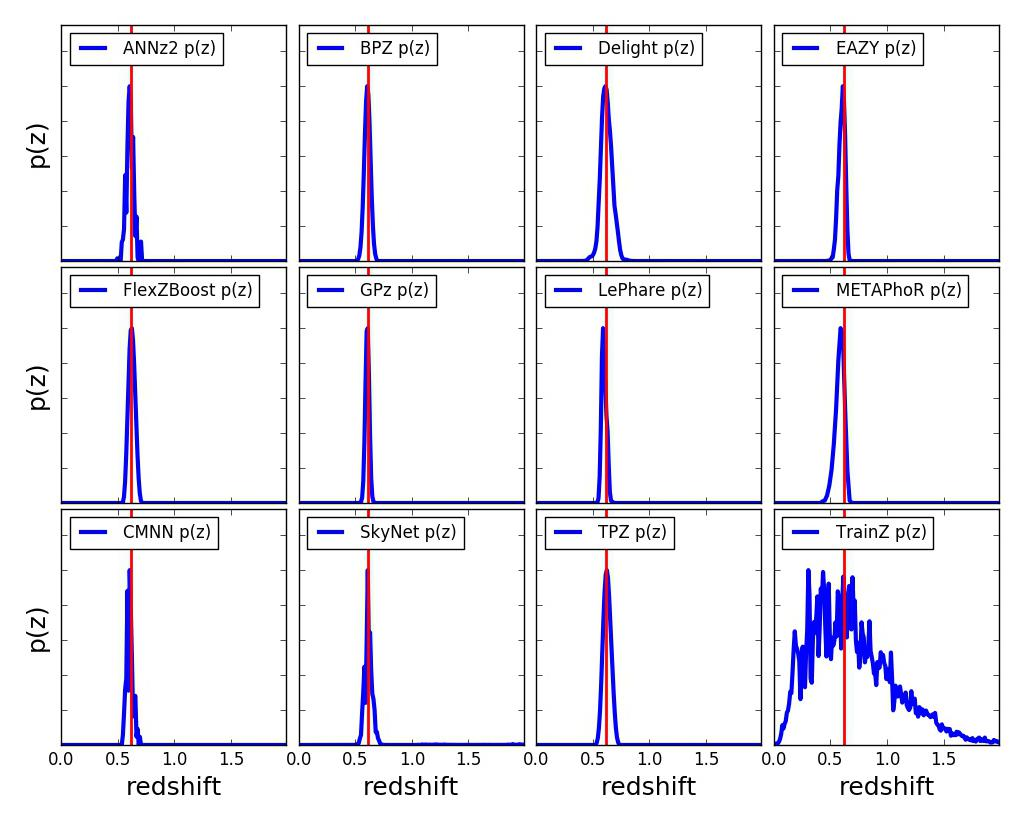
\includegraphics[width=0.49\textwidth]{figures/pzdc1/pz_12codes_261931_noseaborn_crop.jpg}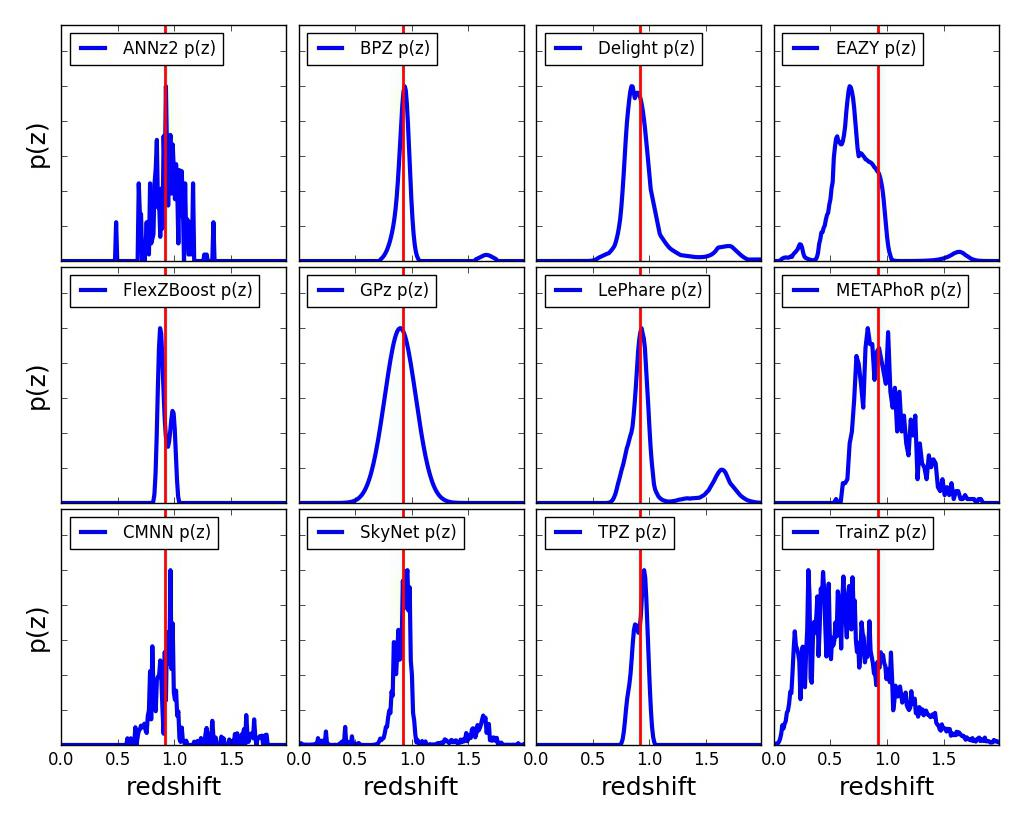
\includegraphics[width=0.49\textwidth]{figures/pzdc1/pz_12codes_471167_noseaborn_crop.jpg}\\
%	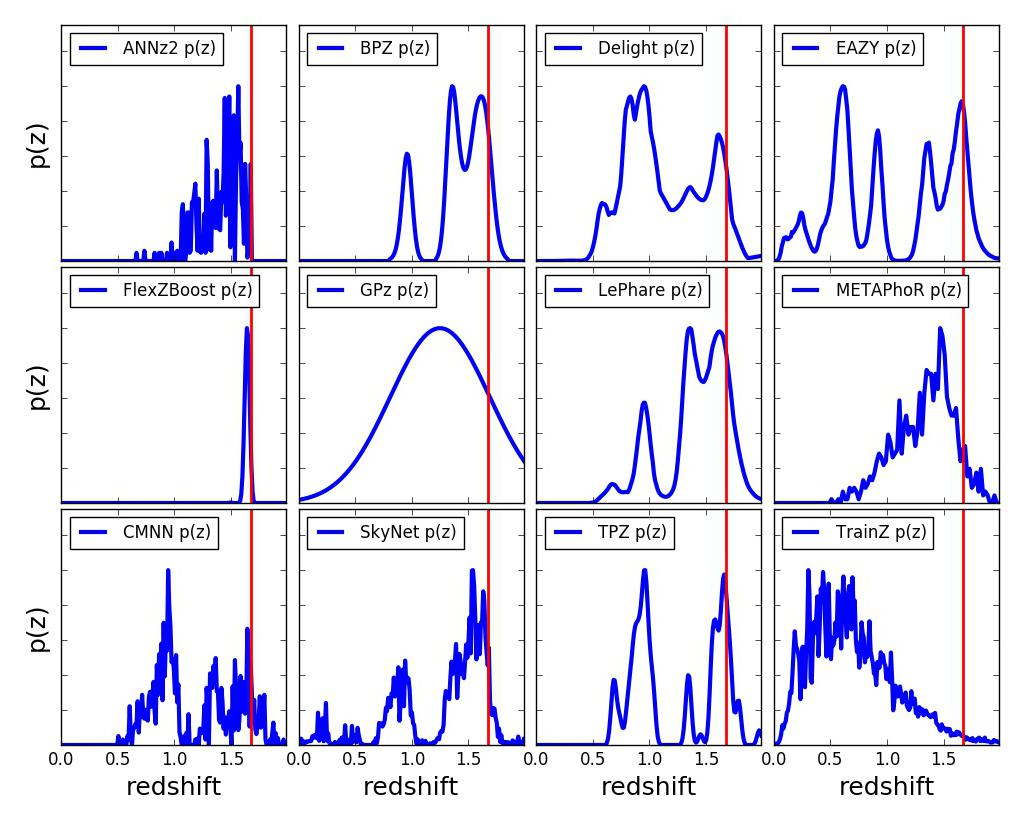
\includegraphics[width=0.49\textwidth]{figures/pzdc1/pz_12codes_713178_noseaborn_crop.jpg}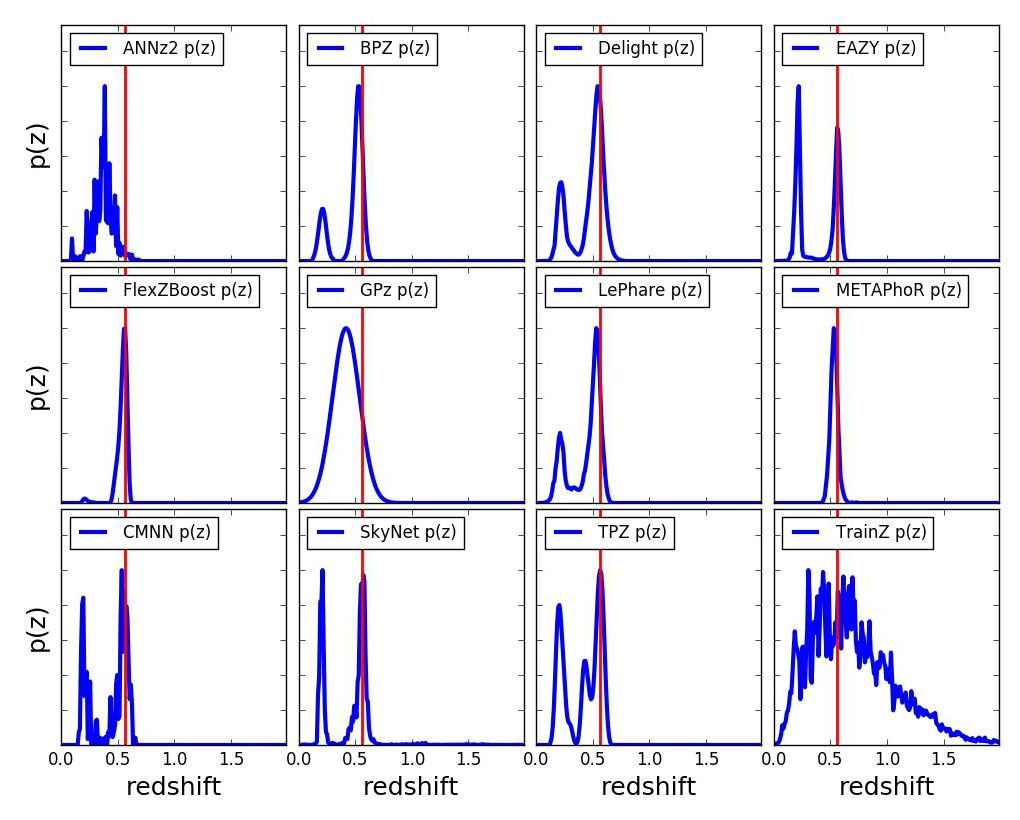
\includegraphics[width=0.49\textwidth]{figures/pzdc1/pz_12codes_982747_noseaborn_crop.jpg}
	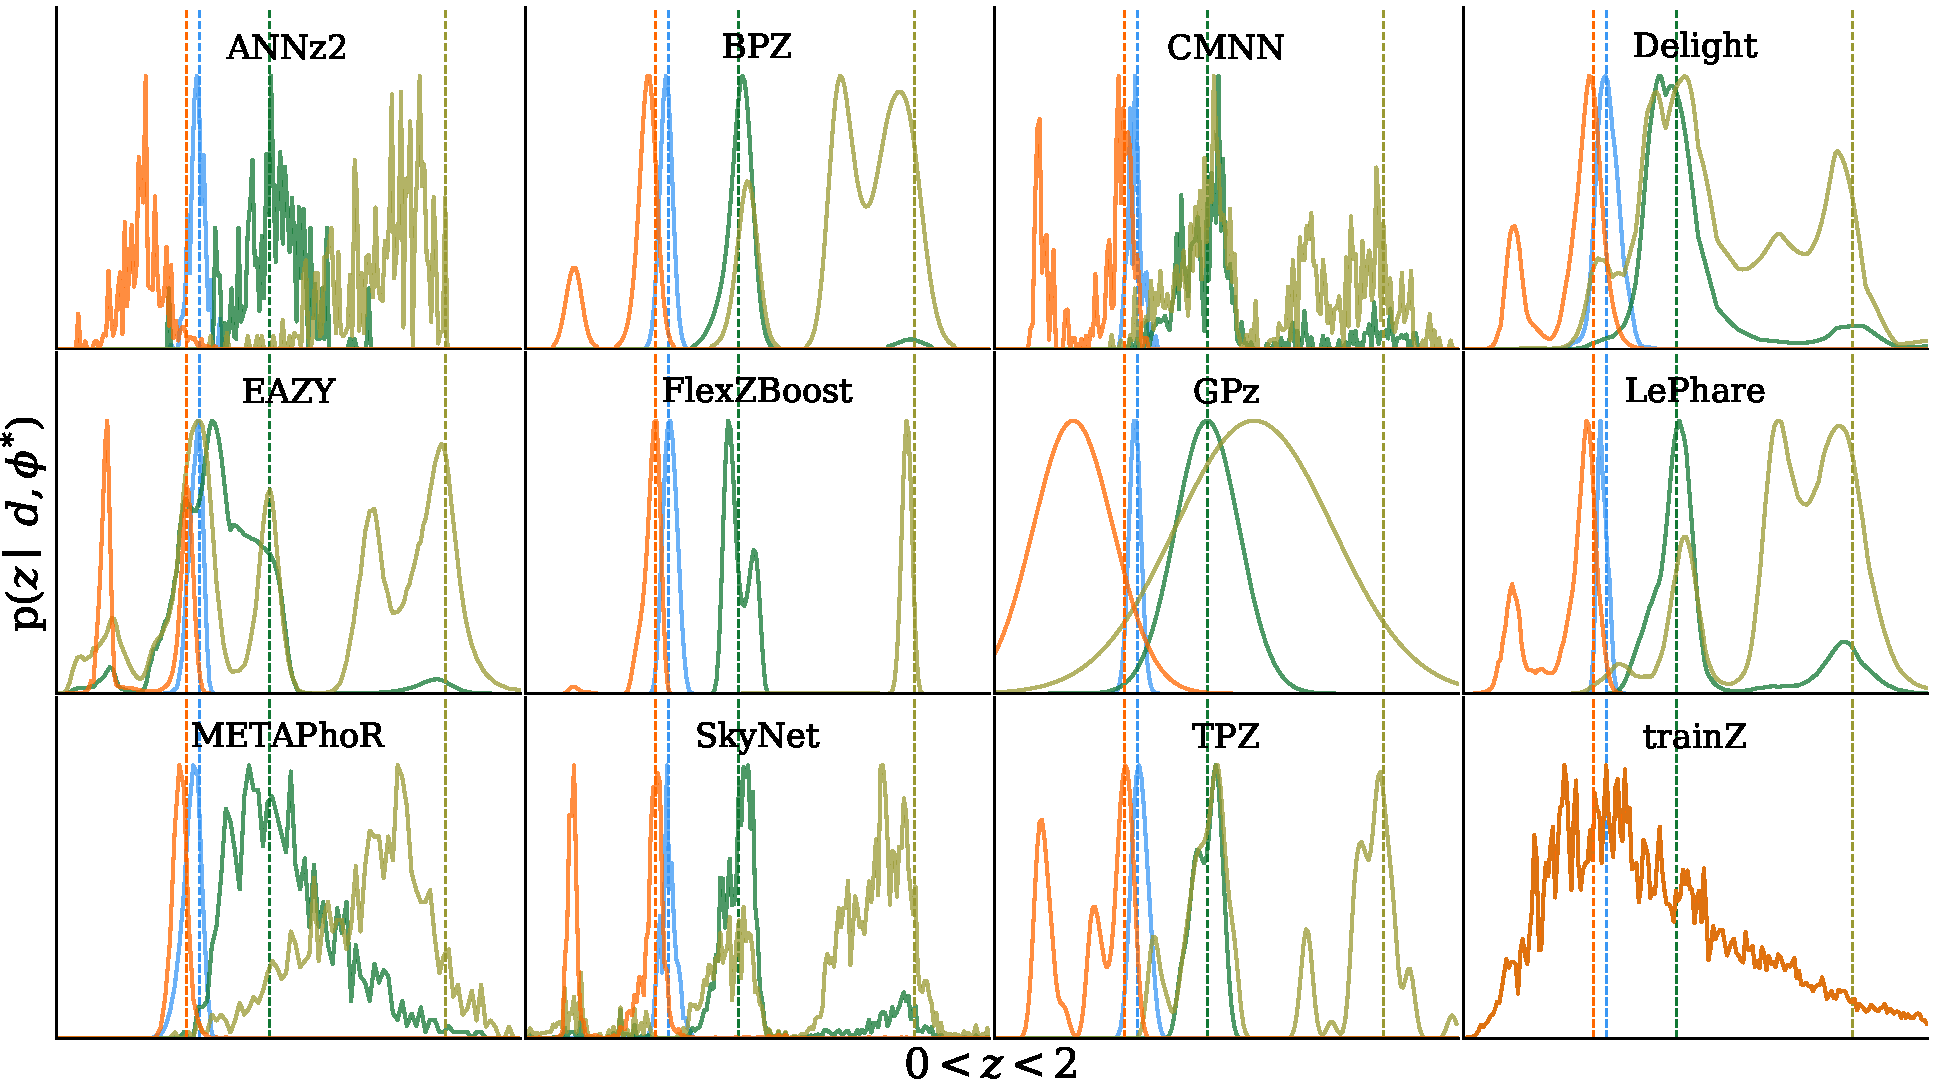
\includegraphics[width=\textwidth]{figures/pzdc1/EXAMPLE_pz_12codes_AIM.pdf}
	\caption{The individual \pzpdf s of four exemplary galaxies (colored curves) produced by the twelve codes (panels) with different true redshifts (vertical lines).
		The \pzpdf s of all codes share some features for the example galaxies due to physical color degeneracies and photometric errors: tight unimodal $p(z)$ (blue), broad unimodal $p(z)$ (green), bimodal $p(z)$ (orange), and complex/multimodal $p(z)$ (yellow).
		The diverse algorithms and implementations induce differences in small-scale structure and sensitivity to physical systematics.}
	\figlabel{fig:pz_examples}
\end{figure*}

The most striking differences between codes are due to small-scale features induced by the interaction between the shared piecewise constant parameterization of $200$ bins $0 < z < 2$ of \Sect{sec:metrics} and the smoothing conditions or lack thereof in each algorithm.
The $\rm{d}z = 0.01$ redshift resolution is sufficient to capture the broad peaks of faint galaxies' \pzpdf s with large photometric errors but is too broad to resolve the narrow peaks for bright galaxies' \pzpdf s with small photometric errors.
This observation is consistent with the findings of \citet[]{Malz:qp} that the piecewise constant parameterization underperforms in the presence of small-scale structures.

However, the shared small-scale features of \annz, \metaphor, \cmnn, and \skynet\ are a result of various weighted sums of the limited number of training set galaxies with colors similar to those of the test set galaxy in question, with behavior closer to classification than regression in the case of \annz.
The settings used on \gpz\ in this work forced broadening of the single Gaussian to cover the multimodal redshift solutions of the other codes.
%Interestingly, while \textsc{ANNz2} shows an abundance of small scale structure in individual $p(z)$ measurements (see Fig.~\ref{fig:pz_examples}), the summed $\hat{N}(z)$ is rather smooth, where the small scale features average out.  This is not the case for the two other codes that show an abundance of substructure in their individual $p(z)$: both \textsc{CMNN} and \textsc{SkyNet} show small scale features both in $p(z)$ and $\hat{N}(z)$.
%In contrast, FlexZBoost, for example, can return estimates on any grid without compression errors as it’s a basis expansion method where only the expansion coefficients need to be stored.
%Codes with a native output format other than the shared piecewise constant binning scheme (or one that can be losslessly converted to it) may suffer from loss of information when converting to it, which could artificially favor some codes over others in a limited number of cases, for example bright galaxies with very narrow $p(z)$ where the true peak falls between grid points.  We will discuss PDF storage in Section~\ref{sec:discussion}.
%Furthermore, the fidelity of photo-$z$ interim posteriors in this format varies with the quality of the photometry.
%Switching to a quantile based parameterization may be more costly computationally, for example template-based codes would need to test more grid point in order to resolve the quantiles for bright galaxies.  However, the computational time for template based codes scales roughly linearly with the number of grid points, so this may be a reasonable thing to implement.
% We will discuss this further in Section~\ref{sec:discussion}.
% \red{someone review this statement to make sure that I'm saying this correctly!}

\subsection{Performance on \pzpdf\ ensembles}
\sectlabel{sec:pitqq}

The histogram of PIT values, QQ plot, and QQ difference plot relative to the ideal diagonal are provided in \Fig{fig:pitqq}, showcasing the biases and trends in the average accuracy of the \pzpdf s for each code.
The high QQ values (more high than low PIT values) of \bpz, \cmnn, \delight, \eazy, and \gpz\ indicate \pzpdf s biased low, and the low QQ values (more low than high PIT values) of \skynet\ and \tpz\ indicate \pzpdf s biased high.

\begin{figure*}
	\centering
	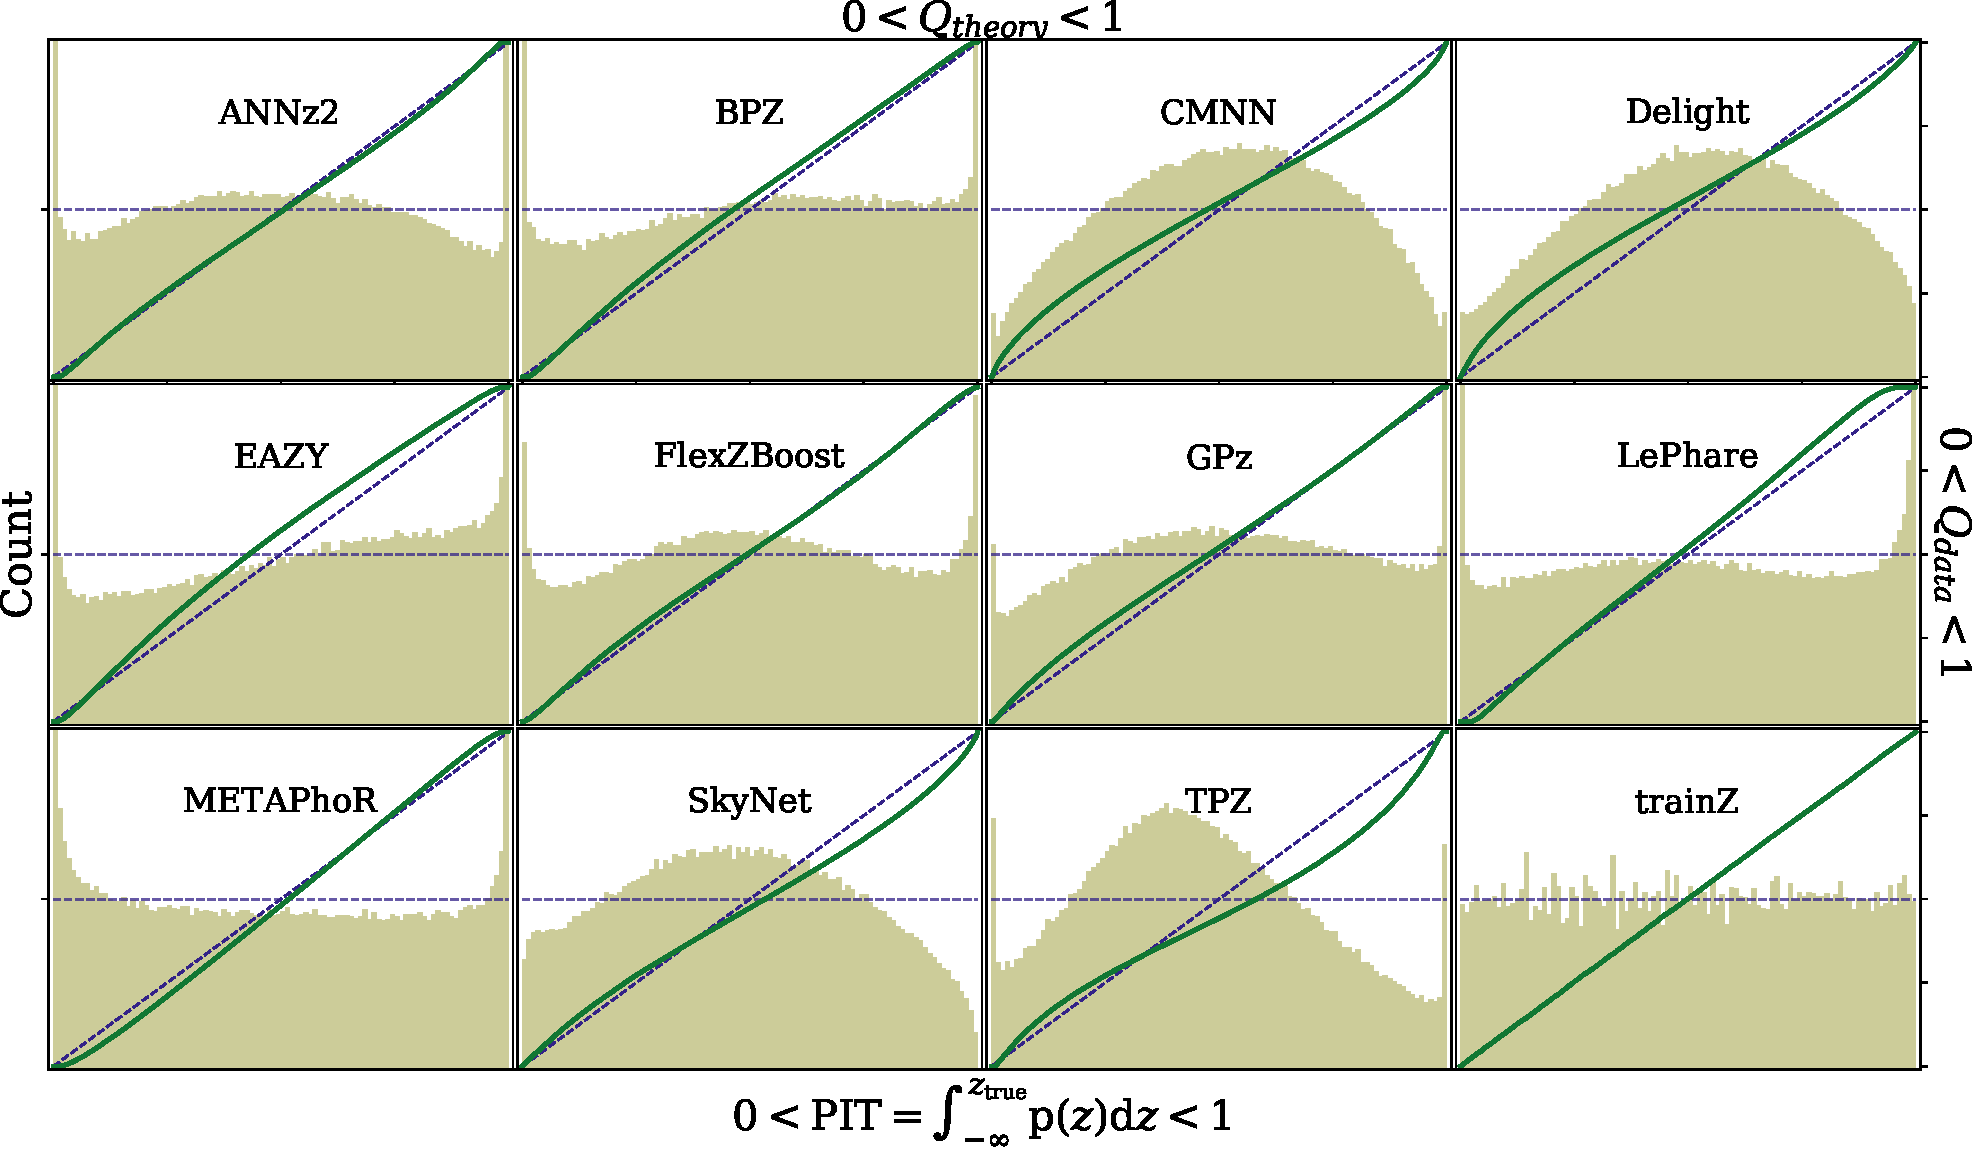
\includegraphics[width=\textwidth]{figures/pzdc1/PITQQcombo_12codes_AIM.pdf}
	\caption{The QQ plot (green curve) and PIT histogram (yellow bars) of the \pzpdf\ codes (panels) along with the ideal QQ (purple dashed diagonal) and ideal PIT (purple dashed horizontal) curves.
%		\aim{Add back the difference of the QQ from the ideal diagonal.}
		The twelve codes exhibit varying degrees of four deviations from perfection: an overabundance of PIT values at the centre of the distribution indicate a catalogue of overly broad \pzpdf s, an excess of PIT values at the extrema indicates a catalogue of overly narrow \pzpdf s, catastrophic outliers manifest as overabundances at PIT values of 0 and 1, and asymmetry indicates systematic bias, a form of model misspecification.}
	\figlabel{fig:pitqq}
\end{figure*}

The PIT histograms of \delight, \cmnn, \skynet, and \tpz\ feature an underrepresentation of extreme values, indicative of overly broad \pzpdf s, while the overrepresentation of extreme values for for \metaphor indicate overly narrow \pzpdf s.
These five codes in particular have a free parameter for bandwidth, which may be responsible for this vulnerability, in spite of the opportunity for fine-tuning with perfect prior information.
\flexzboost's ``sharpening'' parameter (described in \Sect{sec:flexzboost}) played a key role in diagonalizing the QQ plot, indicating a common avenue for improvement in the approaches that share this type of parameter.
On the other hand, the three purely template-based codes, \bpz, \eazy, and \lephare, do not exhibit much systematic broadening or narrowing, which may indicate that complete template coverage effectively defends from these effects.

\begin{table}
	\setlength{\tabcolsep}{2pt}
	\centering
	\caption{The catastrophic outlier rate as defined by extreme PIT values.
		We expect a value of 0.0002 for a proper Uniform distribution.
		An excess over this small value indicates true redshifts that fall outside the non-zero support of the $p(z)$.}
	\tablabel{tab:pitoutlier}
	\begin{tabular}{lc}
		\hline
		\hline
		\Pz\ Code & fraction PIT$<10^{-4}$ or $>$0.9999\\
		\hline
		\annz       & 0.0265\\
		\bpz        & 0.0192\\
		\delight    & 0.0006\\
		\eazy       & 0.0154\\
		\flexzboost & 0.0202\\
		\gpz        & 0.0058\\
		\lephare    & 0.0486\\
		\metaphor   & 0.0229\\
		\cmnn       & 0.0034\\
		\skynet     & 0.0001\\
		\tpz        & 0.0130\\
		\hline
		\trainz     & 0.0002
	\end{tabular}
\end{table}

Though the spikes in the first and last bin of the PIT histogram were cut off in \Fig{fig:pitqq} for visualization, the catastrophic outlier rates are provided in \Tab{tab:pitoutlier}.
As expected, \trainz\ achieves precisely the 0.0002 value expected of an ideal PIT distribution.
\annz, \flexzboost, \lephare, and \metaphor\ have notably high catastrophic outlier rates $> 0.02$, exceeding 100 times the ideal PIT rate, meriting further investigation.

\begin{figure*}
	\centering
	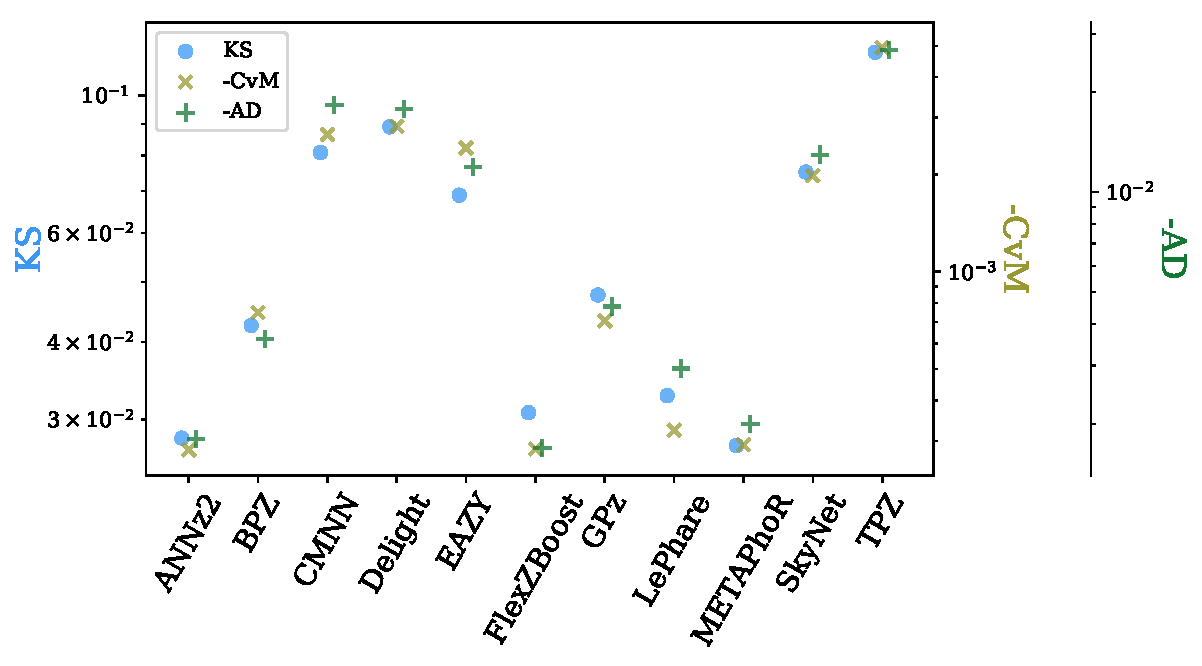
\includegraphics[width=0.74\textwidth]{figures/pzdc1/KSvsCvMvsAD_PIT.pdf}
	\caption{A visualization of the Kolmogorov-Smirnoff (KS, blue $\bullet$), Cramer-von Mises (CvM, yellow $\times$), and Anderson-Darling (AD, green $+$) statistics for the PIT distributions.
		There is generally good agreement between these statistics, with differences corresponding to the codes with outstanding catastrophic outlier rates, a reflection in the differences in how each statistic weights the tails of the distribution.}
	\figlabel{fig:pit_stats}
\end{figure*}

\Fig{fig:pit_stats} displays the values of the KS, CvM, and AD test statistics between the PIT distribution and a uniform distribution $U(0, 1)$, highlighting the relative rather than absolute numbers.
%\red{Can p-values be supplied for each statistic? The statistics themselves are difficult to interpret, other than ``lower is better'' (p-value in skgof was broken, having trouble finding 1-sample KS calculation for uniform distribution)}
\metaphor\ and \lephare\ perform well under the AD but poorly under the KS and CvM due to their high catastrophic outlier rates.
\annz\ and \flexzboost\  are the top scorers under these metrics of the PIT distribution.
\annz's strong performance can be attributed to an aspect of the training process in which training set galaxies with a PIT that more closely matches the percentiles of the DC1 training set's redshift distribution are upweighted; in effect, these quantile-based metrics were part of the algorithm itself that may or may not serve it well under more realistic experimental conditions.

\subsection{Performance on individual \pzpdf s}
\sectlabel{sec:cdelossresults}

The values of the CDE loss statistic of individual \pzpdf\ accuracy are provided in \Tab{tab:cdeloss}.
It is worth noting that strong performance on the CDE loss should imply strong performance on the other metrics, though the inverse is not necessarily true.
Thus the CDE loss is the most effective metric for generic science cases.

\begin{table}  %%% DATA TABLE %%%
	\centering
	\caption{CDE loss statistic of the individual \pzpdf s for each code.
		A lower value of the CDE loss indicates more accurate individual \pzpdf s, with \cmnn\ and \flexzboost\ performing best under this metric.}
	\tablabel{tab:cdeloss}
	\begin{tabular}{lr}
		\hline
		Photo-$z$ Code & CDE Loss \\
		\hline
		\annz 	    & $-6.88$ \\
		\bpz 		    & $-7.82$ \\
		%\textsc{Delight} 	& $-4.06$ \\
		\delight    & $-8.33$\\
		%\textsc{EAZY} 		& $-7.97$ \\
		\eazy       & $-7.07$ \\
		%\textsc{FlexZBoost} & $-11.51$ \\
		\flexzboost & $-10.60$\\
		\gpz		    & $-9.93$ \\
		\lephare 	  & $-1.66$ \\
		\metaphor 	& $-6.28$ \\
		%\textsc{CMNN} 		& $-$ \\
		\cmnn       & $-10.43$ \\
		\skynet 	  & $-7.89$ \\
		\tpz 		    & $-9.55$ \\
		\hline
		\trainz		  & $-0.83$ \\
		%\textsc{Frankenz}	& $-$  \\
		%\hline
	\end{tabular}
\end{table}

This metric is the only one that can appropriately penalize \trainz\ and indicates strong performance for \cmnn\ and \flexzboost, the latter of which is optimized for this metric.
%Empirically, we have found that PIT RMSE is not as closely correlated to CDE loss as it is to the $N(z)$ statistics.

\section{Discussion \& Future Directions}
\sectlabel{sec:discussion}
%(Sam Schmidt, Ofer Lahav, Jeff Newman, Alex Malz, Eve Kovacs, Tony Tyson, Tina Peters)

% If methods can not reach the goals on idealized data, then they will almost surely not meet those same goals when the more complex problems that we expect to arise from real LSST data are included.
% The results presented in this paper enable an evaluation of which algorithms are the most promising moving forward, and potentially point to avenues for improvement.

In contrast with other \pzpdf\ comparison papers that have aimed to identify the ``best'' code for a given survey, we have focused on the somewhat more philosophical questions of how to assess \pzpdf\ methods and how to interpret differences between codes in terms of \pzpdf\ performance.
In \Sect{sec:caution}, we reframe the strong performance of our pathological \pzpdf\ technique, \trainz, as a cautionary tale about the importance of choosing appropriate comparison metrics.
In \Sect{sec:futureexperiments}, we outline the experiments we intend to build upon this study
In \Sect{sec:futuredata}, we discuss the enhancements of the mock data set that will be necessary to enable the future experiments.

\subsection{Interpretation of metrics}
\sectlabel{sec:caution}
%(Alex Malz, Sam Schmidt)

We remind the reader that contributed codes were given a goal of obtaining accurate \pzpdf s, not an accurate stacked estimator of the redshift distribution, so we do not expect the same codes to necessarily perform well for both classes of metrics.
Indeed, the codes were optimized for their interpretation of our request for ``accurate \pzpdf s,'' and we expect that the implementations would have been adjusted had we requested optimization of the traditional metrics of \Sect{sec:moments} and \Sect{sec:pointmetrics}.

Furthermore, our metrics are not necessarily able to assess the fidelity of individual \pzpdf s relative to true posteriors.
Metric-specific performance implies that we may need multiple \pzpdf\ approaches tuned to each metric in order to maximize returns over all science cases in large upcoming surveys.

The \trainz\ estimator of \Sect{sec:trainz}, which assigns every galaxy a \pzpdf\ equal to $N(z)$ of the training set, is introduced as an experimental control or null test to demonstrate this point via \textit{reductio ad absurdum}.
Because our training set is perfectly representative of the test set, $N(z)$ should be identical for both sets down to statistical noise.
\textit{We make the alarming observation that \trainz\ outperforms all codes on the PIT-based metrics, and all but one code on the $N(z)$ based statistics.}
%\textit{Explain the connection between \trainz\ and these metrics.}

The CDE loss and point estimate metrics appropriately penalize \trainz's naivete.
As shown in \Sect{sec:pointmetrics}, \trainz ~has identical $ZPEAK$ and $ZWEIGHT$ values for every galaxy, and thus the \pz\ point estimats are constant as a function of true redshift, i.e. a horizontal line at the mode and mean of the training set distribution respectively.
The explicit dependence on the individual posteriors in the calculation of the CDE loss, described in \Sect{sec:cdelossresults}, distinguishes this metric from those of the \pzpdf\ ensemble and stacked estimator of the redshift distribution, despite their prevalence in the \pz\ literature.

% While looking at one, or even most of our metrics would have given the impression that this estimator was nearly optimal, red flags in CDE loss and point estimates reveal the problems.
%[more caution on over-reliance on metrics, and making sure that metrics test all of what you want] \red{this definitely still needs work}
In summary, context is crucial to defending against deceptively strong performers such as \trainz; \textbf{the best \pzpdf\ method is the one that most effectively achieves our science goals}, not the one that performs best on a metric that does not reflect those goals.
In the absence of a single scientific motivation or the information necessary for a principled metric definition, we must consider many metrics and be critical of the information transmitted by each.
% As stated earlier, science applications may be sensitive to individual \pzpdf s, \pzpdf\ ensembles, \pz\ point estimates, or science-specific statistics like $\hat{N}(z)$.
% We must be aware of that the optimal method for one is not necessarily optimal for the other, and in fact several photo-$z$ algorithms may be necessary in the final cosmological analysis in order to satisfy the requirements of all science use cases.
% The example of the simple \trainz\ estimator described in Section~\ref{sec:caution} shows a simple model with a $p(z)$ that is unrealistic for individual objects can still score very well on many of our metrics.
% It is important to look at {\it all} metrics, and keep in mind what information each metric conveys.
%\aim{[reiterate the meaning of $p(z)$ and the goal -- emphasize finding ``best'' code in terms of impact of assumptions underlying the method \textit{or} establishing methodology for the realistic case of biased prior information and other science goals]}
%\red{[the challenges faced in this project]}
%\red{mention z$<$2, missing some important degeneracies, new sim will go to higher z}
%\red{no quality cuts included, could identify outliers, but could also induce biases}
%\red{[how optimization defined has impact, here we optimized p(z), not n(z), could be science-case specific if stringent requirements are needed, though that may be a computational/storage challenge if too many use cases needed.]}
%\red{some discussion of output parameterization, limitations of 200 point fixed grid, in future switch to something like quantiles (cite qp paper)}

\subsection{Extensions to the experimental design}
\sectlabel{sec:futureexperiments}

%\begin{enumerate}
%\item \red{the combination of codes}
%\item \red{$p(z,\alpha)$}
%\item \red{tomographic analysis later on}
%\red{this paper deals with training, future papers will also explore calibration via cross-correlation methods}
%\end{enumerate}
%\red{mention the SRM once again, say that the plans are extensive, but we do have a plan and a rough timeline.}

The work presented in this paper is only a first step in assessing \pzpdf\ approaches and moving toward an improved photometric redshift estimator.
Here we discuss the next steps for subsequent investigations.

This initial paper explored code performance in idealized conditions with perfect catalog-based photometry and representative training data.
A top priority for a follow-up study is to test realistic forms of incomplete, erroneous, and non-representative template libraries and training sets as well as the impact of other forms of external priors that must be ingested by the codes, major concerns in \citet{Newman:2015, Masters:2017}.
We plan to perform a full sensitivity analysis on a realistically incomplete training set of spectroscopic galaxies, modeling the performance of spectrographs, emission-line properties, and expected signal-to-noise to determine which potential training set galaxies are most likely to be excluded.
In addition to outright redshift failures we will model the inclusion of a small number of high-confidence yet false redshifts due to emission line misidentification or noise spikes.

\Sect{sec:moments} only addresses the stacked estimator of the redshift distribution of the entire galaxy catalogue rather than subsets in bins, tomographic or otherwise.
The effects of tomographic binning scheme will be explored in a dedicated future paper, including propagation of redshift uncertainties in a set of fiducial tomographic redshift bins in order to estimate impact on cosmological parameter estimation.

%\red{[are there any references for this?  I remember Gary Bernstein talking about this at a photo-z workshop in Japan, but I don't know that it was published.  I believe Michael Troxel has discussed this as well.]}
%\item \red{cosmological parameters in DC2}
%\item \red{mention z$<$2, missing some important degeneracies, new sim will go to higher z}
%\red{no quality cuts included, could identify outliers, but could also induce biases}

Sequels to this study will also address some shortcomings of our experimental procedure.
The fixed redshift grid shared between the codes may have unfairly penalized codes with a different native parameterization, as precision is lost when converting between formats.
Performance on sharply peaked \pzpdf s may have been suppressed across all codes due to the insufficient resolution of the redshift grid.
In light of the results of \citet[]{Malz:qp}, in future analyses we plan to switch from a fixed grid to the quantile parameterization or to permit each code to use its native storage format under a shared number of parameters.

\subsection{Realistic mock data}
\sectlabel{sec:futuredata}

To make optimal use of the \lsst\ data for cosmological and other astrophysical analyses of the Science Roadmap, future investigations that build upon this one will require a more sophisticated set of galaxy photometry and redshifts.
%\item \red{inclusion of photometric errors, image based effects, blending, lensing, sky, mask, etc...}
This initial paper explored a data set that was constructed at the catalog level, with no inclusion of the complications that come from measuring photometry from images.
Future data challenges will move to catalogs constructed from mock images, including the complications of deblending, sensor inefficiencies, and heterogeneous observing conditions, all anticipated to affect the measured colours of \lsst's galaxy sample \citep{Dawson:2016}.

The DC1 galaxy SEDs were linear combinations of just five basis SED templates, but a next generation of data for \pzpdf\ investigations must include a broader range of physical properties.
Though we only considered $z < 2$ here, \lsst\ 10-year data will contain $z > 2$ galaxies, plagued by fainter apparent magnitudes and anomalous colours due to stellar evolution.
A subsequent study must also have a data set that includes low-level active galactic nuclei (AGN) features in the SEDs, which perturb colours and other host galaxy properties.
An observational degeneracy between the Lyman break of a $z \sim 2-3$ galaxy from the Balmer break of a $z \sim 0.2-0.3$ galaxy is a known source of catastrophic outliers \citep{Massarotti:2001} that was not effectively included in this study.
To gauge the sensitivity of \pzpdf\ estimators to catastrophic outliers, our data set must include realistic high-redshift galaxy populations.

% In this study we have not accounted for the presence of Active Galactic Nuclei (AGN) contributions to galaxy fluxes.
% In some cases, AGN will be easily identified from the colors and morphologies, i.e. the case of the brightest quasars where the nuclear activity outshines the host galaxy, and numerous studies have utilized color selection to create large samples of quasars \citep[e.g.][]{Richards:06,Maddox:08,Richards:15}.
% In current deep fields, similar in depth to what we expect from \lsst, variability information and multi-wavelength data have been critical to not only identify AGN dominated galaxies, but also obtain more accurate photometric redshifts \citep[e.g][]{Salvato:11}.
%
% In addition to AGN dominated galaxies, those with lower levels of nuclear activity present a more insidious problem, where AGN features may not be apparent, but the colours and other host galaxy properties are perturbed relative to galaxies with an inactive nucleus.
% In such cases, the presence of the AGN may induce a bias if the template SEDs or empirical datasets do not include low-level AGN counterparts.
% For LSST, we will need to identify and obtain accurate photometric redshifts of all types of AGN for a range of science goals, whether it is to eliminate such objects from cosmology experiments, or to use them with confidence, all the way through to understanding galaxy evolution and the role that AGN may play in influencing galaxy properties over cosmic time.

% A promising route to classifying and obtaining accurate photometric redshifts for the AGN population is by combining machine learning with template-fitting techniques, as has recently been demonstrated by \citet{Duncan:18} for radio-selected AGN.
% This is because AGN are relatively easy to obtain spectroscopic redshifts for over all redshifts due to the strong emission lines that they exhibit, allowing very good training sets for machine learning algorithms to use.
% Whereas for those galaxies where the AGN is sub-dominant the galaxy templates are still adequate for obtaining reasonable photometric redshifts.

% In addition to these improvements, the \lsstdesc \Pz\ Working Group plans to look at all potential methods to combine the results from multiple \pzpdf\ codes to improve accuracy, similar to the work presented in \citet{Dahlen:13,Carrascokind:14,Duncan:18}.
% Taking advantage of multiple algorithms that use observables in slightly different ways has shown promise, however we must be very conscious of whether a potential combination properly treats the covariance between the methods, given that they are estimating quantities based on the same underlying observables.
% Several science cases wish to estimate physical quantities along with redshift, for example galaxy stellar mass and star formation rate.
% Proper joint estimation of redshift and physical quantities requires an in depth understanding of galaxy evolution, and progress on accurate bivariate redshift probability distributions will go hand in had with progress on understanding galaxies themselves.
% Parameterization and storage of a complex 2-dimensional probability surface for potentially billions of galaxies (or even subsets of hundreds of thousand of particular interest) pose a potential challenge.
% These issues will be examined in another future paper.

% Finally, while this paper and future papers discussed above focus on photometric redshift codes and estimating accurate \pzpdf s from training data, we plan a separate, but complementary, project to examine calibration of the resultant redshifts via spatial cross-correlations \citep{Newman:2008}, which will be explored in a separate series of future papers.
The overarching plan describing everything laid out in this section is described in more detail in the \desc\ Science Roadmap\footref{lsstdesc_srm}).

\section{Conclusion}
\sectlabel{sec:conclusion}
%(Sam Schmidt, Ofer Lahav, Jeff Newman, Alex Malz, Eve Kovacs, Tony Tyson, Tina Peters)

This paper compares twelve \pzpdf\ codes under controlled experimental conditions of representative and complete prior information to set a baseline for an upcoming sensitivity analysis.
This work isolates the impact on metrics of \pzpdf\ accuracy due to the estimation technique as opposed to the complications of realistic physical systematics of the photometry.
Though the mock data set of this investigation did not include true \pz\ posteriors for comparison, \textbf{we interpret deviations from perfect results given perfect prior information as the imprint of the implicit assumptions underlying the estimation approach}.

We evaluate the twelve codes under science-agnostic metrics both established and emerging to stress-test the ensemble properties of \pzpdf\ catalogues derived by each method.
In appendices, we also present metrics of point estimates and a prevalent summary statistic of \pzpdf\ catalogues used in cosmological analyses to enable the reader to relate this work to studies of similar scope.
We observe that no one code dominates in all metrics, and that the standard metrics of \pzpdf s and the stacked estimator of the redshift distribution can be gamed by a vacuously wrong procedure that asserts the prior over the data.
We emphasize to the \pz\ community that \textbf{metrics used to vet \pzpdf\ methods must be scrutinized to ensure they correspond to the quantities that matter to our science}.

\section*{Appendices}
\addcontentsline{toc}{section}{Appendices}
\renewcommand{\thesubsection}{\Alph{subsection}}

\subsection{Evaluation of the redshift distribution}
\label{sec:moments}
%(Alex Malz)

Perhaps the most popular application of \pzpdf s is the estimation of the overall redshift distribution $N(z)$, a quantity that enters some cosmological calculations and the true value of which is known for the DC1 data set and will be denoted as $\tilde{N}(z)$.
In terms of the prior information provided to each method, the true redshift distribution satisfies the tautology $\tilde{N}(z) = p(z \vert I_{D})$ due to our experimental set-up; because the DC1 training and template sets are representative and complete, $I_{D}$ represents a prior that is also equal to the truth.
In this ideal case of complete and representative prior information, the method that would give the best approximation to $\hat{N}(z)$ would be one that neglects all the information contained in the photometry $\{d_{i}\}_{N_{tot}}$ and gives every galaxy the same \pzpdf\ $\hat{p}_{i}(z) = \tilde{N}(z)$ for all $i$; the inclusion of any information from the photometry would only introduce noise to the optimal result of returning the prior.
This is the exact estimator, \trainz, that we have described in \Sect{sec:trainz}, and which will serve as an experimental control.

\subsubsection{Metrics of the stacked estimator of the redshift distribution}
\label{sec:stackedmetrics}

Though alternatives exist \citep{Malz:chippr}, ``stacking'' according to
\begin{equation}
\label{eq:stacked}
\hat{N}^{H}(z) \equiv \frac{1}{N_{tot}}\ \sum_{i}^{N_{tot}}\ \hat{p}^{H}_{i}(z)
\end{equation}
is the most widely accepted method for obtaining $\hat{N}^{H}(z)$ as an estimator of the redshift distribution from \pzpdf s derived by a method $H$.
Though we do not endorse the use of the stacked estimator of the redshift distribution, we use it under the untested assumption that the response of our metrics of $\hat{N}^{H}(z)$ will be analogous to the same metrics applied to a principled estimator of the redshift distribution.

As $N(z)$ is itself a univariate PDF, we apply the metrics of the previous sections to it as well.
We additionaly calculate the first three moments
\begin{equation}
\eqlabel{eq:moment}
\langle z^{m}\rangle \equiv \int_{-\infty}^{\infty} z^{m} N(z) dz
\end{equation}
of the estimated redshift distribution $\hat{N}^{H}(z)$ for each code and compare them to the moments of the true redshift distribution $\tilde{N}(z)$.
Under the assumption that the stacked estimator is unbiased, a superior method minimizes the difference between the true and estimated moments.

\subsubsection{Performance on the stacked estimator of the redshift distribution}
\label{sec:stackedmetrics_results}

\Fig{fig:nz} shows the stacked estimator $\hat{N}(z)$ of the redshift distribution for each code compared to the true redshift distribution $\tilde{N}(z)$, where the stacked estimator has been smoothed for each code in the plot using a kernel density estimate (KDE) with a bandwidth chosen by Scott's Rule \citep{Scott:1992} in order to minimize visual differences in small-scale features; the quantiative statistics, however, are calculated using the empirical CDF which is not smoothed.

\begin{figure*}
	\centering
	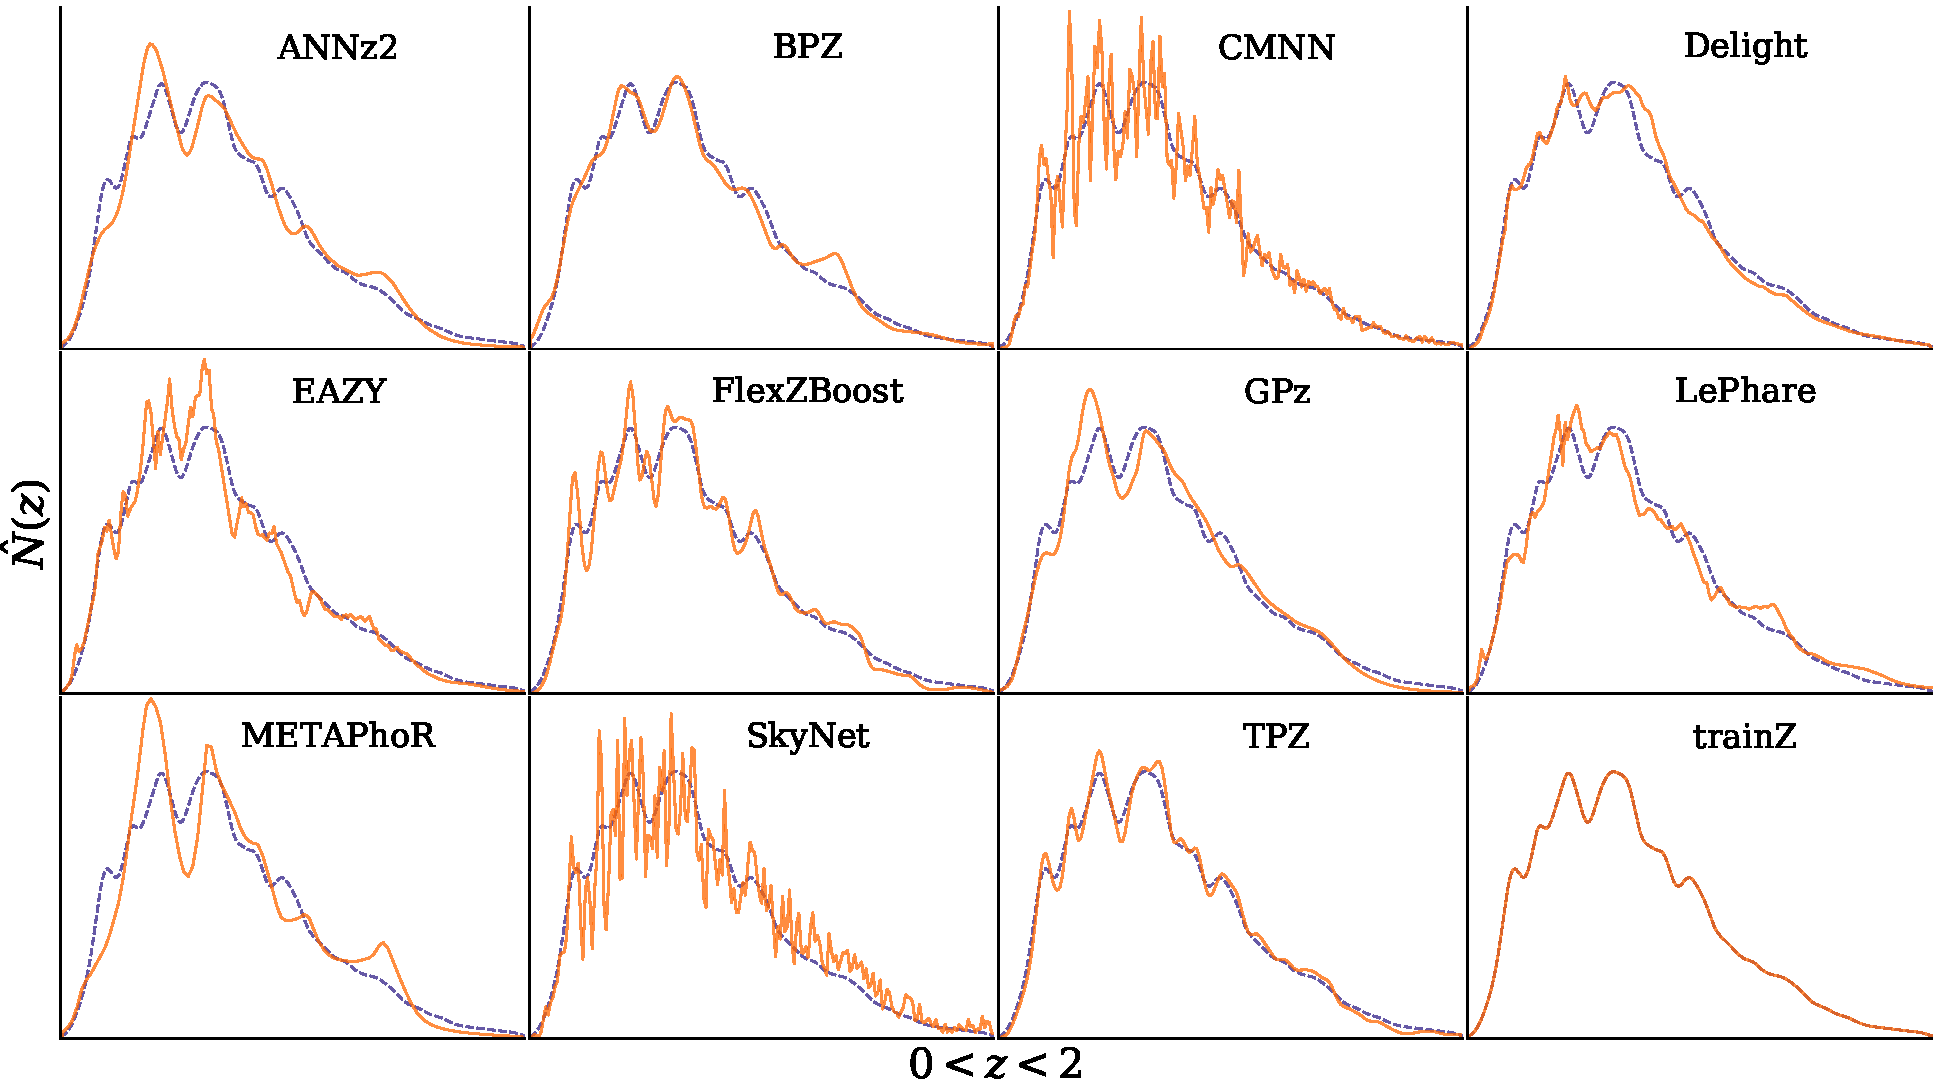
\includegraphics[width=\textwidth]{figures/pzdc1/NZsumplot_AIM.pdf}
	\caption{The smoothed stacked estimator $\hat{N}(z)$ of the redshift distribution (orange) produced by each code (panels) compared to the true redshift distribution $\tilde{N}(z)$ (purple dashed).
		Varying levels of agreement are seen among the codes, with the smallest deviations for \cmnn, \flexzboost, \tpz, and \trainz.}
	\figlabel{fig:nz}
	%\aim{Arguably this could also be clarified by showing the true $n'(z)$ once and then differences from it for each cod's stacked estimator\dots}\scc{what if we plot the difference between true and stacked rather than soverposing the two lines? Sam please do not hate me.}
\end{figure*}

Many of the codes, including all the model-fitting approaches and \annz, \gpz, \metaphor, and \skynet\ from the data-driven camp, overestimate the redshift density at $z \sim 1.4$.
This behavior is a consequence of the $4000 \rm{\AA}$ break passing through the gap between the $z$ and $y$ filters, which induces a genuine discontinuity in the $z - y$ colour as a function of redshift that can sway the \pzpdf\ estimates in the absence of bluer spectral features.

\annz, \gpz, and \metaphor\ show signs of overtraining, estimating enhanced peaks and diminished troughs relative to the training set, an obstacle that may be overcome with adjustment of the implementation.

As expected, \trainz\ perfectly recovers the true redshift distribution: as the training sample is selected from the same underlying distribution as the test set, the redshift distributions are identical, up to Poisson fluctuations due to the finite number of sample galaxies.
\cmnn\ is also in excellent agreement for similar reasons: with a representative training sample of galaxies spanning the colour-space, the sum of the colour-matched neighbour redshifts should return the true redshift distribution.
\flexzboost\ and \tpz\ also perform superb recovery of the true redshift distribution, with only a slight deviation at $z \sim 1.4$.
Our metrics, however, cannot discern whether these four approaches, as well as \delight, are spared the $z \sim 1.4$ degeneracy in $\hat{N}(z)$ because they have more effectively used information in the data or if the impact is simply washed out by the stacked estimator's effective average over the test set galaxy sample.
See \Sect{sec:pointmetrics} for further discussion of the $z \sim 1.4$ issue.

\Fig{fig:nz_stats} shows the quantitative Kolmogorov-Smirnoff (KS), Cramer-Von Mises (CvM), and Anderson Darling (AD) test statistics for each of the codes for the $\hat{N}(z)$ based measures.
%\red{Can p-values be supplied for each statistic? The statistics themselves are difficult to interpret, other than ``lower is better'' (no, p-values are very difficult to compute for non-uniform distributions)}
The stacked estimators of the redshift distribution for \cmnn\ and \trainz\ best estimate $\tilde{N}(z)$ under these metrics, and the only codes that do especially poorly are \eazy, \lephare, \metaphor, and \skynet.
It is unsurprising that \cmnn\ scores well, as with a near perfectly representative training set means that choosing neighbouring points in color/magnitude space should lead to excellent agreement in the final $\hat{N}(z)$ estimate.

\begin{figure*}
	\centering
	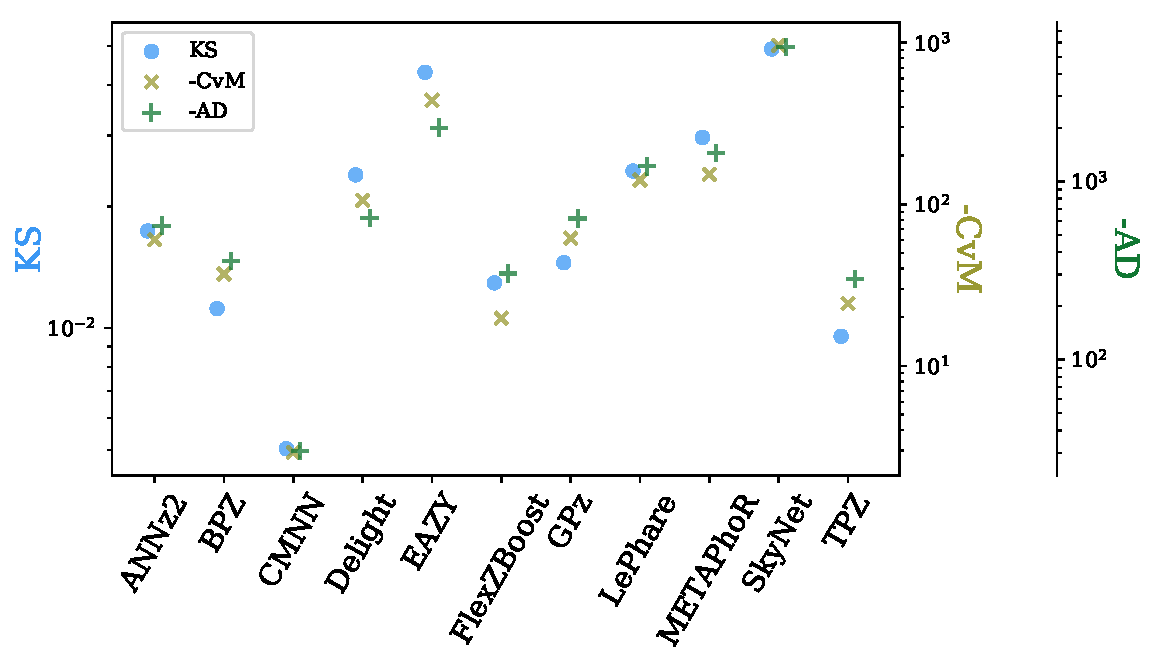
\includegraphics[width=0.74\textwidth]{figures/pzdc1/KSvsCvMvsAD_Nz.pdf}
	\caption{A visualization of the Kolmogorov-Smirnoff (KS, blue $\bullet$), Cramer-von Mises (CvM, yellow $\times$), and Anderson-Darling (AD, green $+$) statistics for the $\hat{N}(z)$ distributions.
		We make the reassuring observation that these related statistics do not disagree significantly with one another.
		\cmnn\ performs comparably well to \trainz, the control case, while \skynet\ scores poorly due to an overall bias in its redshift predictions.}
	\figlabel{fig:nz_stats}
\end{figure*}

It is, however, surprising that \tpz\ does well on $\hat{N}(z)$ given its poor performance on the ensemble \pzpdf s, especially knowing that \tpz\ was optimized for \pzpdf\ ensemble metrics rather than the stacked estimator of the redshift distribution.
A possible explanation is the choice of smoothing parameter chosen during validation, which affects \pzpdf\ widths as well as overall redshift bias and could be modified to improve performance under the \pzpdf\ metrics.

The first three moments of the stacked $\hat{N}(z)$ distribution relative to the empirical estimate of the truth distribution are given in \Tab{tab:moments}.
Accuracy of the moments varies widely between codes, raising concerns about the propagation to cosmological analyses.
%\red{[mention that we are calculating moments for the entire sample, will look at fiducial tomographic bins in a follow-up paper (unless group and reviewers realy think we should include in this paper.]}
%\red{FlexZBoost has some of the best $n(z)$ statistics, but the moments are not good.  Why is this?  Is it the over/underprediction of the high redshift part of the distribution?  Discuss this after talking with Rafael.}

\begin{table}
	\begin{center}
	\setlength{\tabcolsep}{2pt}
	\caption{Moments of the stacked estimator $\hat{N}(z)$ of the redshift distribution.
		Most of the codes considered recover the moments of $\tilde{N}(z)$}
	\tablabel{tab:moments}
	\begin{tabular}{lccc}
		\hline
		\hline
		\multicolumn{4}{l}{Moments of $\hat{N}(z)$} \\
		\hline
		Estimator  & mean       & variance    & skewness \\
		Empirical ``truth'' & 0.701 & 0.630 & 0.671  \\
		\hline
		\annz       & 0.702      & 0.625      & 0.653    \\
		\bpz        & 0.699      & 0.629      & 0.671    \\
		\delight    & 0.692      & 0.609      & 0.638    \\
		\eazy       & 0.681      & 0.595      & 0.619    \\
		\flexzboost & 0.694      & 0.610      & 0.631    \\
		\gpz        & 0.696      & 0.615      & 0.639    \\
		\lephare    & 0.718      & 0.668      & 0.741    \\
		\metaphor   & 0.705      & 0.628      & 0.657    \\
		\cmnn       & 0.701      & 0.628      & 0.667    \\
		\skynet     & 0.743      & 0.708      & 0.797    \\
		\tpz        & 0.700      & 0.619      & 0.643    \\
		\hline
		\trainz	    & 0.699 		 & 0.627 	    & 0.666 \\
	\end{tabular}
\end{center}
\end{table}

\skynet\ exhibits redshift bias in \Fig{fig:nz} and is a clear outlier in the first moment of $\hat{N}(z)$ in \Tab{tab:moments}.
The \skynet\ algorithm employs a random subsampling of the training set without testing that the subset is representative of the full population, and the implementation used here does not upweight rarer low- and high-redshift galaxies, as in \citet{Bonnett:15}, suggesting a possible cause that may be addressed in future work.

\subsection{\Pz\ point estimation and metrics}
\label{sec:allpointmetrics}

While this work assumes that science applications value the information of the full \pzpdf, we present conventional metrics of \pz\ point estimates as a quick and dirty diagnostic tool and to facilitate direct comparisons to historical studies.

\subsubsection{Reduction of \pzpdf s to point estimates}
\label{sec:pointest}

Though we acknowledge that many of the codes can also return a native \pz\ point estimate, we put all codes on equal footing by considering two generic \pz\ point estimators, the mode $z_{PEAK}$ and main-peak-mean $z_{WEIGHT}$ \citep{Dahlen:13}, a weighted mean within the bounds of the main peak, as identified by the roots of $p(z) - 0.05 \times z_{PEAK}$.
Though $z_{WEIGHT}$ neglects information in a secondary peak of a, say, bimodal distribution, it avoids the pitfall of reducing the \pzpdf\ to a redshift between peaks where there is low probability.

\subsubsection{Metrics of \pz\ point estimates}
\sectlabel{sec:pointmetrics}

We calculate the commonly used point estimate metrics of the overall intrinsic scatter, bias, and catastrophic outlier rate, defined in terms of the standard error $e_{z} \equiv (z_{PEAK} - z_{\rm true}) / (1 + z_{\rm true})$.
Because the standard deviation of the \pz\ residuals is sensitive to outliers, we define the scatter in terms of the Interquartile Range (IQR), the difference between the 75th and 25th percentiles of the distribution of $e_{z}$, imposing the scaling $\sigma_{\rm IQR} = \rm{IQR} / 1.349$ to ensure that the area within $\sigma_{\rm IQR}$ is the same as that within one standard deviation from a standard Normal distribution.
We also resist the effect of catastrophic outliers by defining the bias $b_{z}$ as the median rather than mean value of $e_{z}$.
The catastrophic outlier rate $f_{\rm out}$ is defined as the fraction of galaxies with $e_{z}$ greater than $\max(3 \sigma_{\rm IQR}, 0.06)$.
For reference, Section 3.8 of the \lsst\ Science Book \citep{Abell:09} uses the standard definitions of these parameters, given in Table~\ref{intro:tab:tab:lsstsrd}.
%\begin{itemize}
%	\item RMS scatter $\sigma < 0.02 (1 + z_{\rm true})$
%	%\scc{actually the SB reports in page 75 that the goal of 0.02 is for the RMS of $\frac{\sigma_{z}}{(1+z)}$ while we are using IQR}
%	\item bias $b_{z} < 0.003$ %\scc{in page 518 of the SB is clearly reported that the mean is expected to be less than 0.003 in our case we have defined as bias the median and not the mean }
%	\item catastrophic outlier rate $f_{\rm out} < 10\%$ %\scc{clearly the number of outliers since are defined above $3\sigma$ strictly depends on the sigma definition, in the science book it seems to refer to the RMS of the $e_z$ distribution even ef it could be the standard deviation, but again I don't think it refers to IQR, therefore we could not consider exactly this numbers as reference.}
%	%\red{I am going off of conversations with Zeljko and how we {\it actually} computed the metrics in the Science Book (I have the scripts).  You are correct that several of these are slightly different than actually stated in the Science Book, or where the Science Book does not use very precise language as to what was done to compute the RMS or define the bias.  We can also cut out those specifics, or maybe say Ivezic private communication, maybe?  Also $\sigma_{z}$ defined in terms of IQR is exactly equivalent to the standard deviation when scaled by 1.349 for a Gaussian distribution, so the numbers are appropriate to cite in this context.  IQR is just a more robust way of calculating sigma for a distribution with outliers.--SJS }
%	%\scc{I am very sorry I am not saying that IQR is not fine, I want to keep the IQR my concerns are related to the notation and the \textit{reader understanding}, if I wrote $\sigma$ somewhere in a table the reader will understand for sure that is the traditional standard deviation (a lot of people skips the indicators definition for the \textit{obvious} ones), I am suggesting to replace the notation $\sigma$ with the notation $\sigma_{IQR}$ (or something like this) to avoid any confusion, and also to change from $bias$ to $median$ for the same reason. I agree that say Ivezic private communication could be better.}
%	.
%\end{itemize}

\subsubsection{Comparison of \pz\ point estimate metrics}
\label{sec:pointmetrics_results}

\Fig{fig:pz_pointestimates} shows both point estimates forall codes  both $z_{PEAK}$ and $z_{WEIGHT}$.
Point density is shown with mixed contours to emphasize that most of the galaxies do fall close to the $z_{phot} = z_{spec}$ line, while points trace the details of the catastrophic outlier populations.

\begin{figure*}
	\centering
	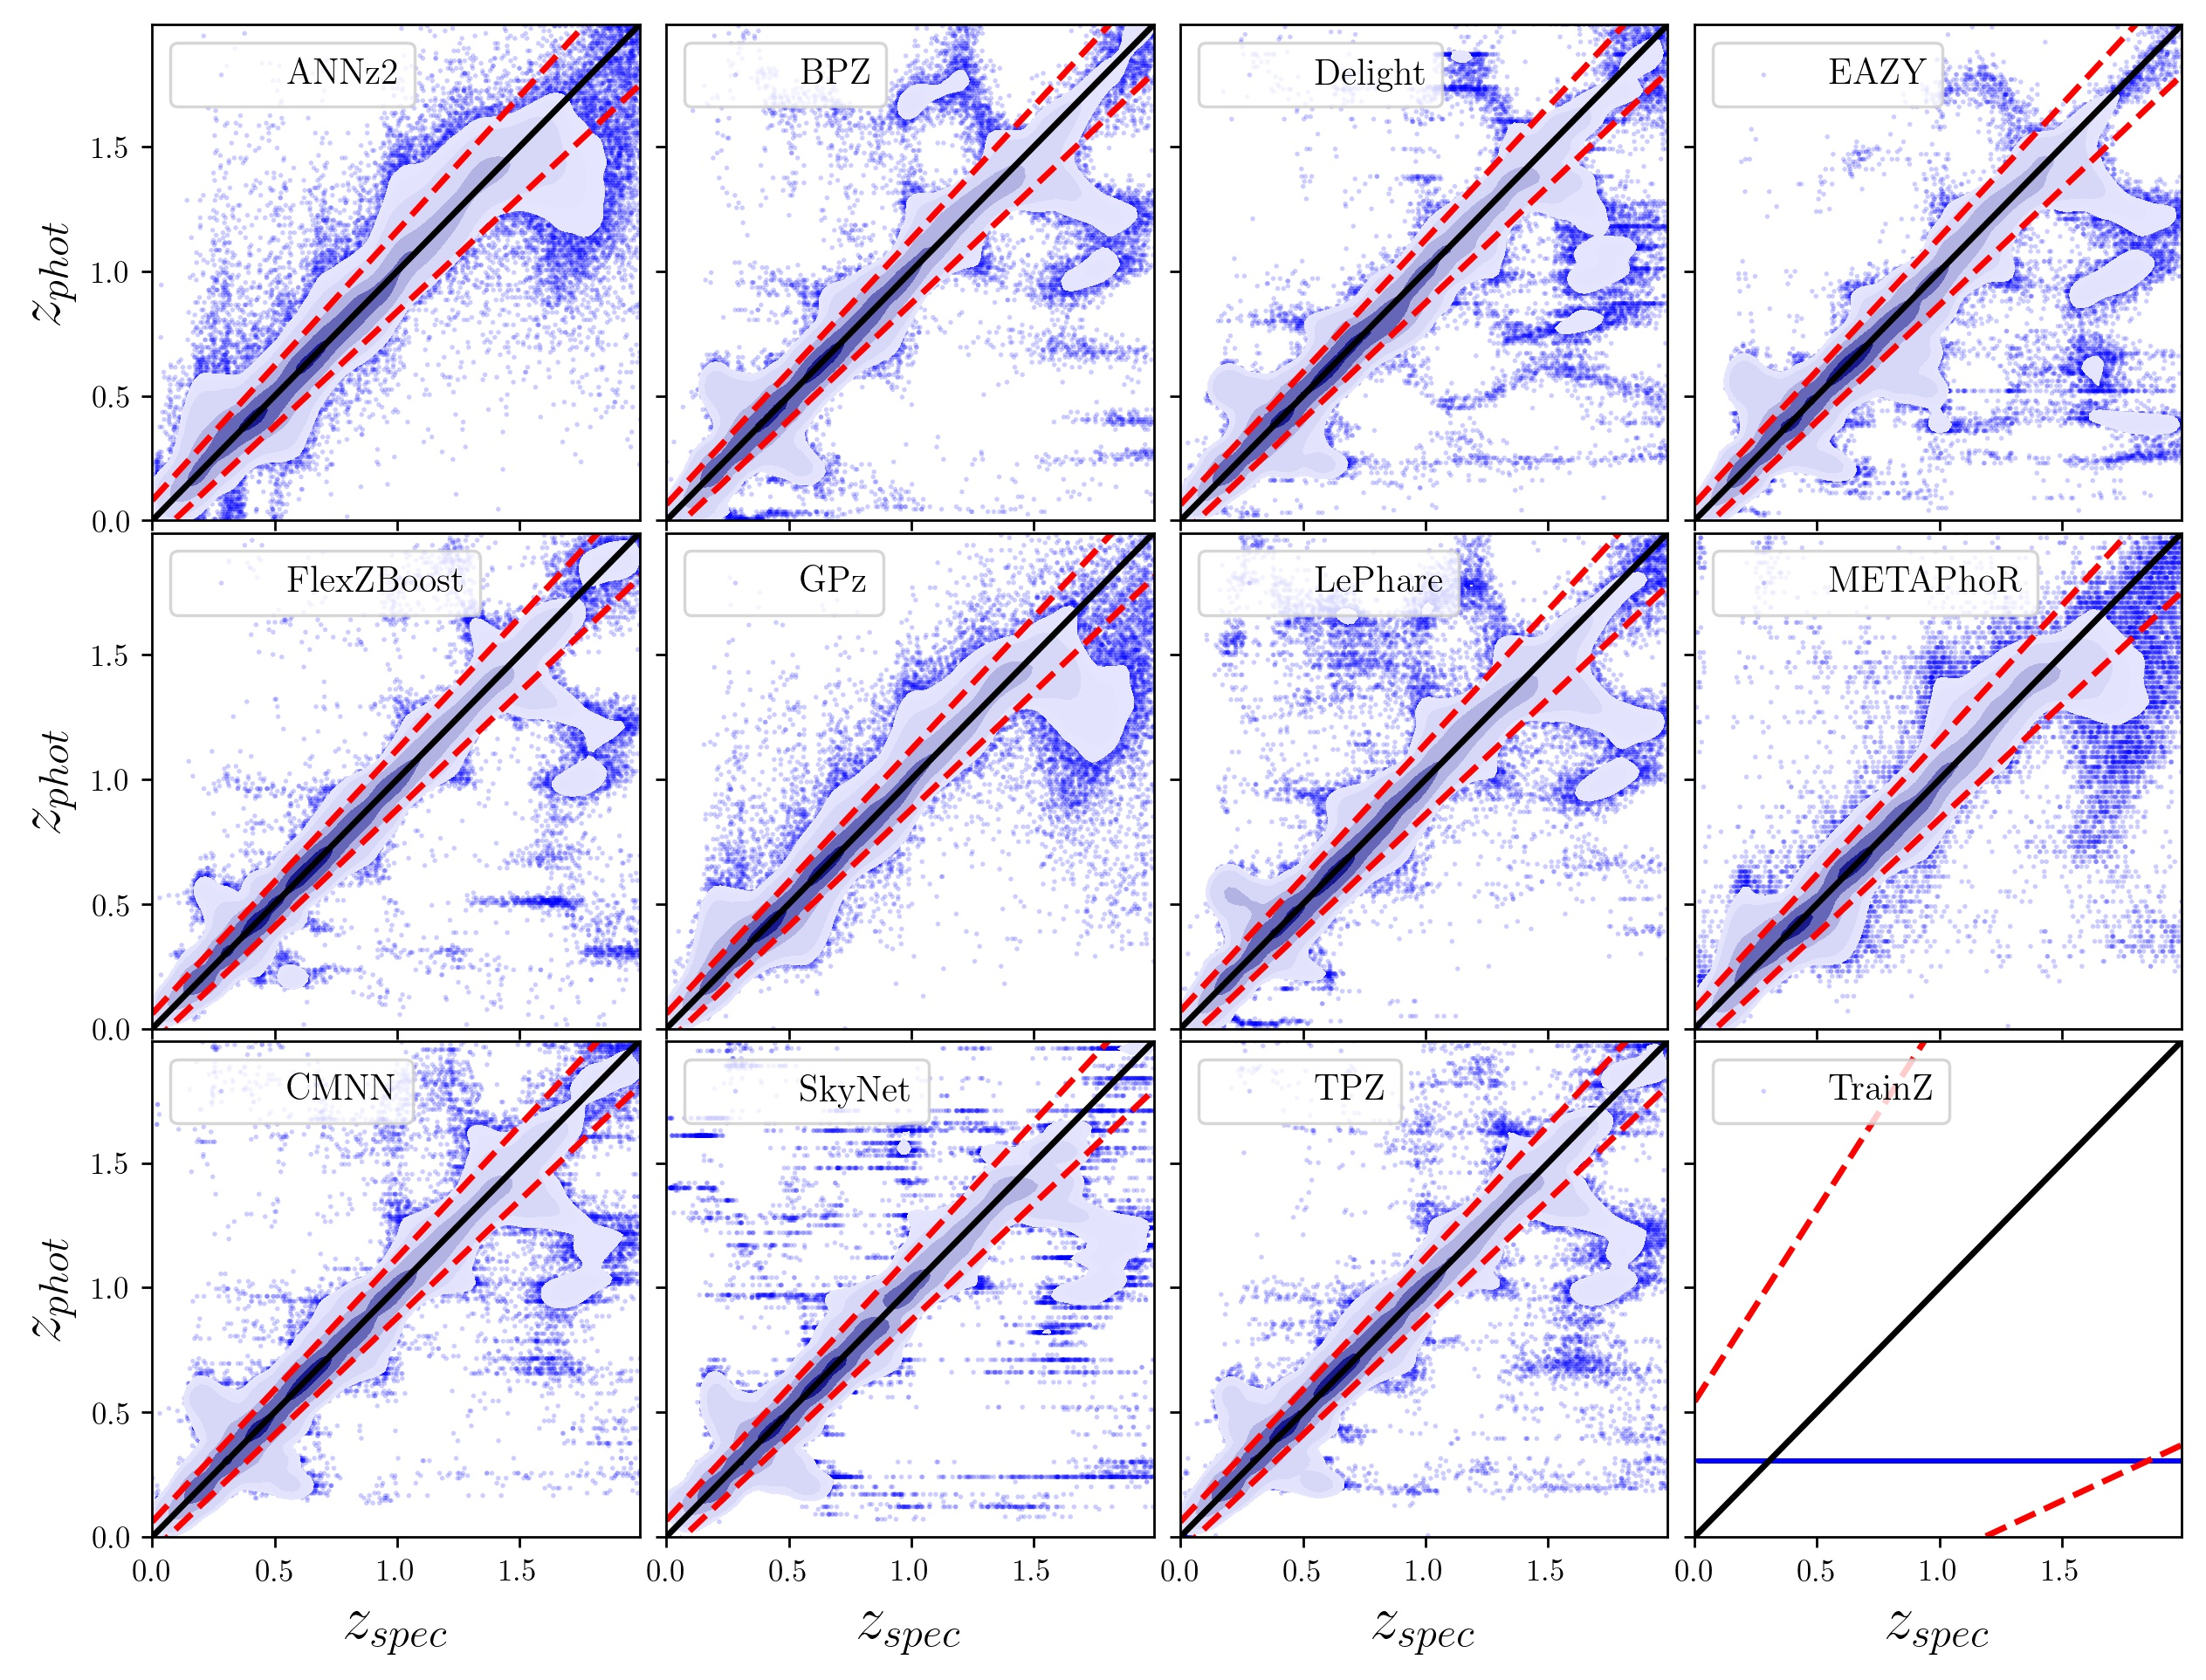
\includegraphics[width=0.49\textwidth]{figures/pzdc1/ZPEAK_szpz_threecolumn_12codes_navy_lowalpha.jpg}
	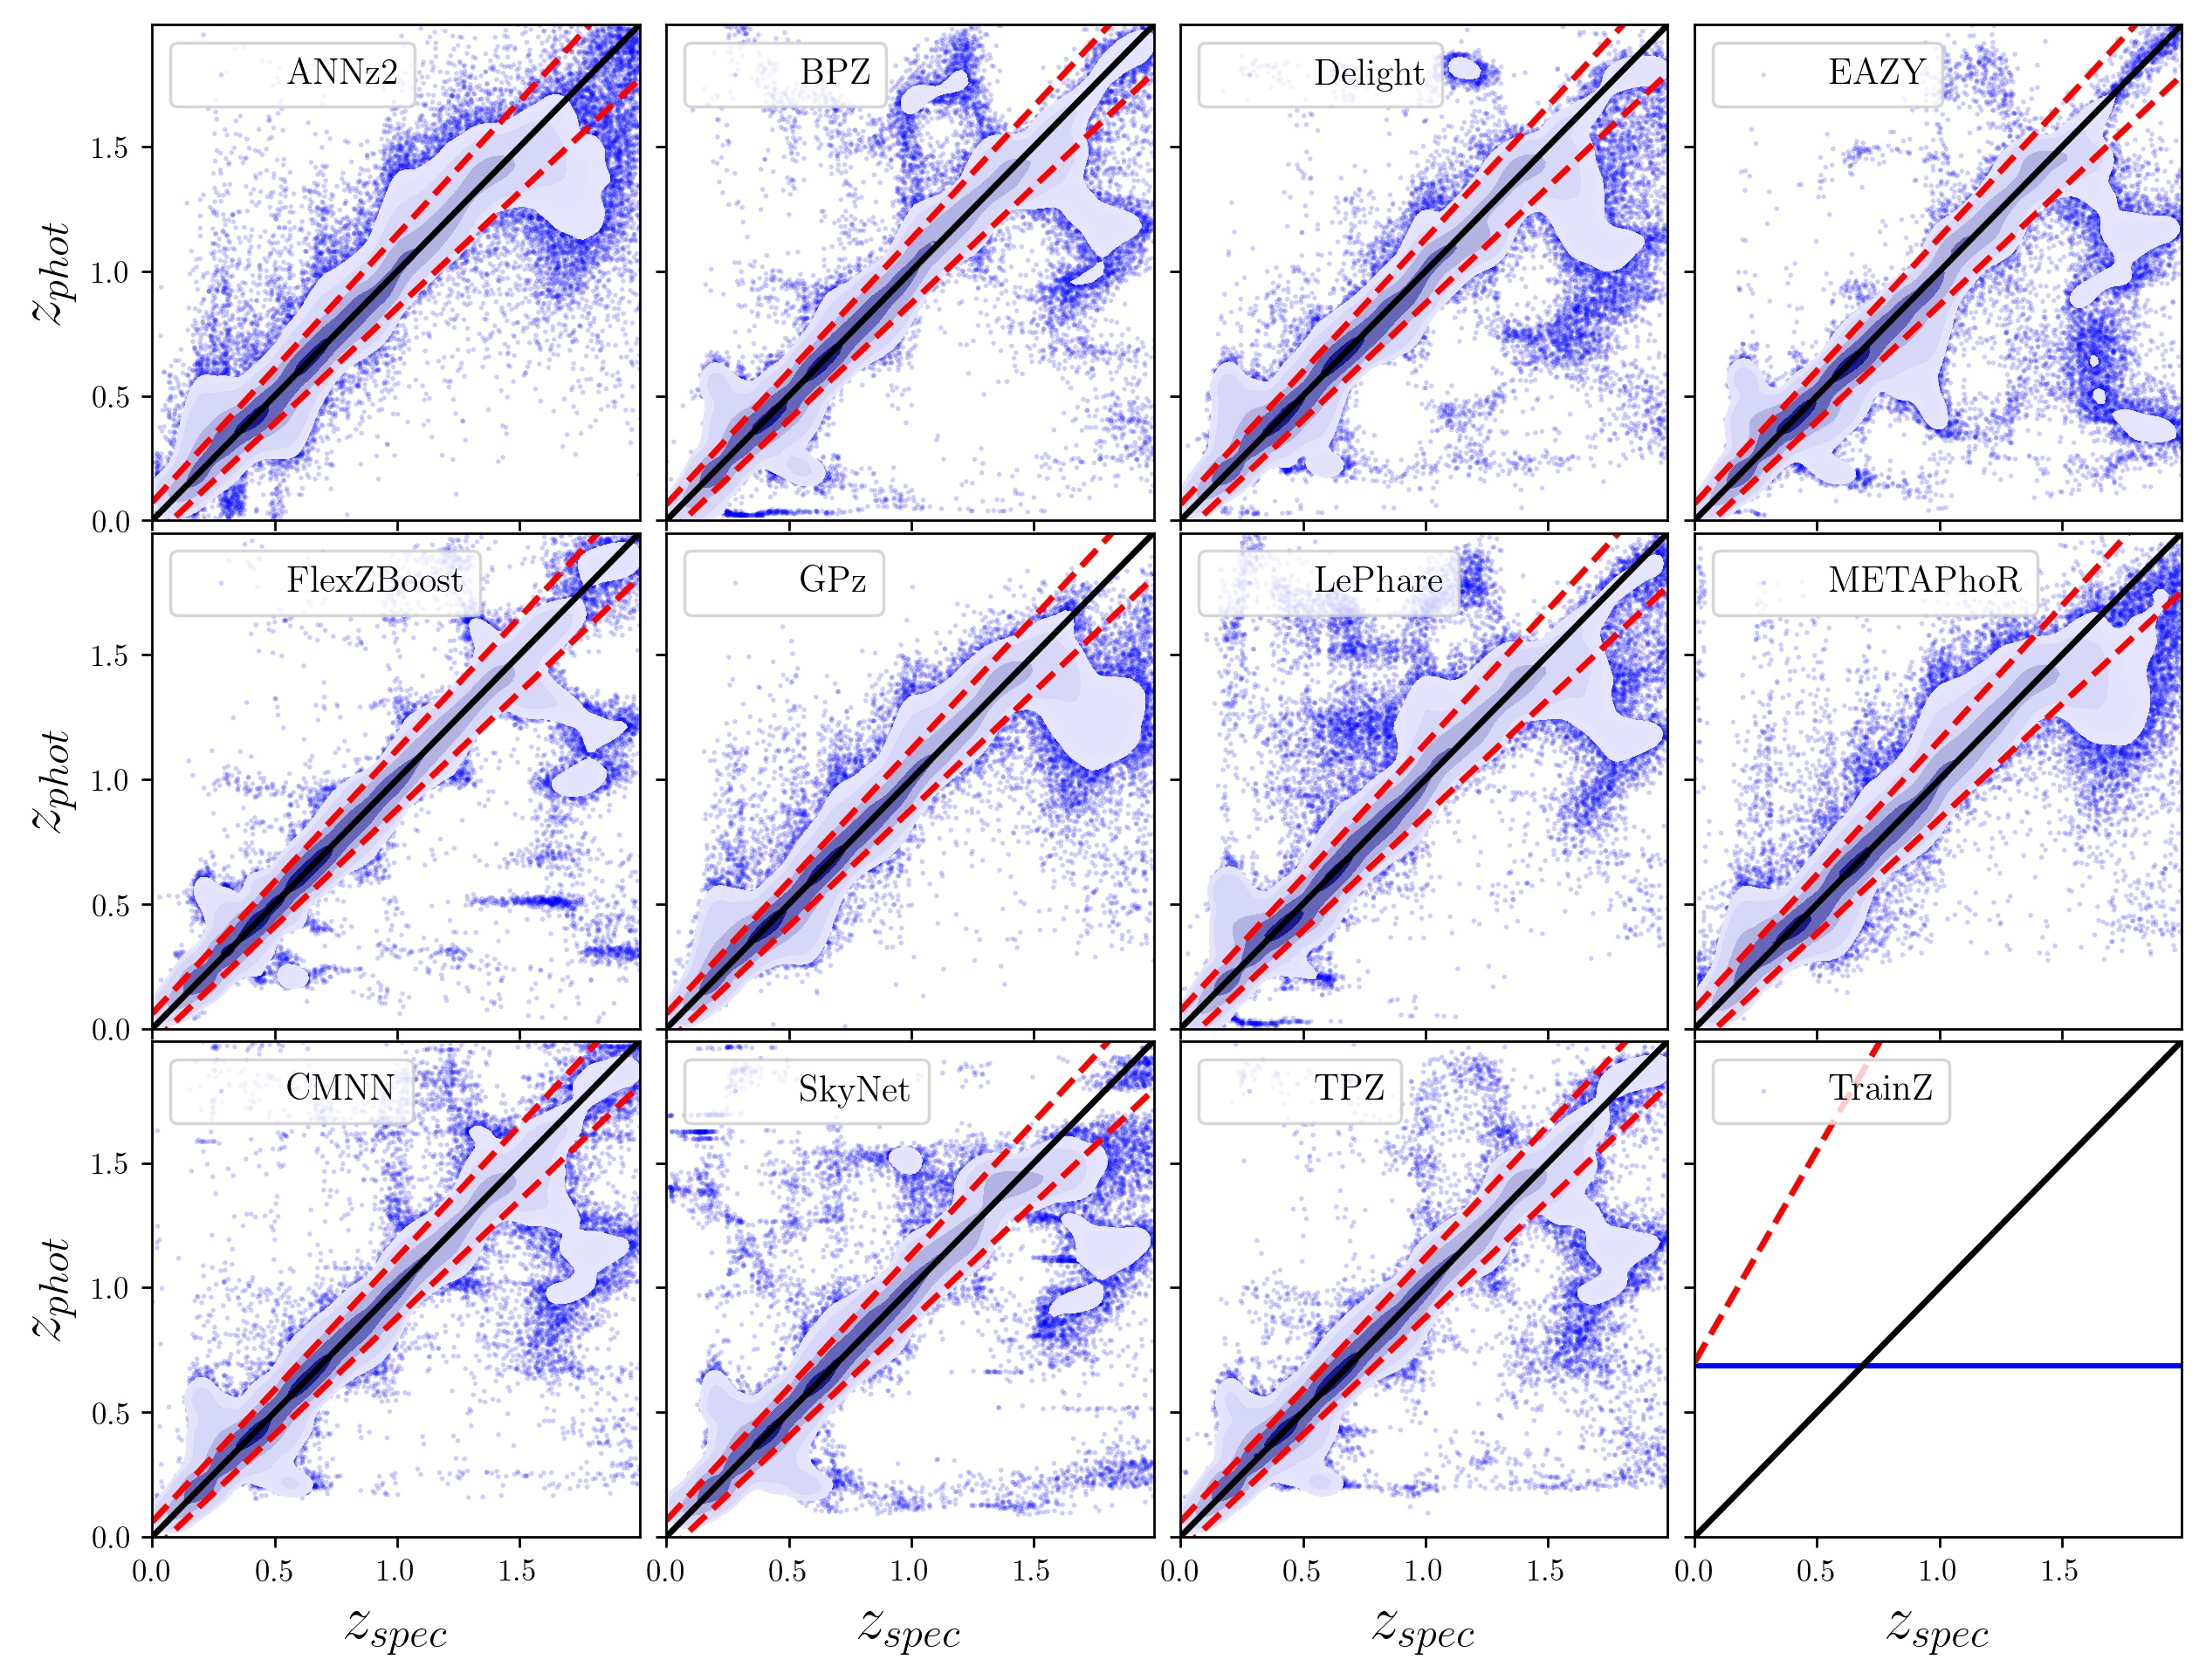
\includegraphics[width=0.49\textwidth]{figures/pzdc1/ZWEIGHT_szpz_threecolumn_12codes_navy_lowalpha.jpg}
	\caption{The density of \pz\ point estimates (contours) reduced from the \pzpdf s with outliers (blue) beyond the outlier cutoff (red dashed lines), via the mode ($z_{PEAK}$, left panel) and main-peak-mean ($z_{WEIGHT}$, right panel).
		The \trainz\ estimator (lower right sub-panels) has a shared $z_{PEAK}$ and $z_{WEIGHT}$ for the entire test set galaxy sample.
	\aim{Overhaul these plots for readability.}}
	\figlabel{fig:pz_pointestimates}
\end{figure*}

The finite grid spacing of the \pzpdf s induces some discretization in $z_{PEAK}$.%, particularly for \skynet.
The features perpendicular to the $z_{phot} = z_{spec}$ line are due to the $4000 \rm{\AA}$ break passing through the gaps between adjacent filters.% and logically are more prominent for template-based codes
Even the strongest codes feature populations far from the $z_{phot} = z_{spec}$ line representing a degeneracy in the space of colours and redshifts.
% While use of the full information available via $p(z)$ mitigates their impact, a full understanding of the outlier population is critical for LSST science, particularly in tomographic applications.
%\red{I forget what exactly I was trying to say here, if someone else wants to take a crack at this it might be helpful --SJS}
%\scc{may be worth to say that the usage of further bands could mitigate this effect by removing the degeneration  usually induced from emission lines moving across different filters?}

\begin{table*}
	\begin{center}
		\caption{\Pz\ point estimate statistics}\tablabel{tab:pointestimates}
		\begin{tabular}{lcccccc}
			\hline
			\hline
			&            & $Z_{PEAK}$  &          &  & $Z_{WEIGHT}$          &\\
			\hline
			\Pzpdf\ Code       & $\frac{\sigma_{IQR}}{(1+z)}$ & median  & \multicolumn{1}{|p{0.75cm}|}{\centering outlier \\fraction} & $\frac{\sigma_{IQR}}{(1+z)}$ & median & \multicolumn{1}{|p{0.75cm}|}{\centering outlier \\fraction}\\
			\hline
			\annz     & 0.0270  &  0.00063  & 0.044      & 0.0244  &  0.000307  & 0.047  \\
			\bpz       & 0.0215  & -0.00175  & 0.035      & 0.0215  & -0.002005  & 0.032 \\
			\delight   & 0.0212  & -0.00185  & 0.038      & 0.0216  & -0.002158  & 0.038 \\
			\eazy      & 0.0225  & -0.00218  & 0.034      & 0.0226  & -0.003765  & 0.029 \\
			\flexzboost& 0.0154  & -0.00027  & 0.020      & 0.0148  & -0.000211  & 0.017 \\
			\gpz       & 0.0197  & -0.00000  & 0.052      & 0.0195  &  0.000113  & 0.051 \\
			\lephare   & 0.0236  & -0.00161  & 0.058      & 0.0239  & -0.002007  & 0.056 \\
			\metaphor  & 0.0264  &  0.00000  & 0.037      & 0.0262  &  0.001333  & 0.048 \\
			\cmnn        & 0.0184  & -0.00132  & 0.035      & 0.0170  & -0.001049  & 0.034 \\
			\skynet    & 0.0219  & -0.00167  & 0.036      & 0.0218  &  0.000174  & 0.037 \\
			\tpz       & 0.0161  &  0.00309  & 0.033      & 0.0166  &  0.003048  & 0.031 \\
			\hline
			\trainz	   & 0.1808  &  -0.2086  & 0.000	  & 0.2335  & 0.022135  & 0.000\\
		\end{tabular}
	\end{center}
\end{table*}

The intrinsic scatter, bias, and catastrophic outlier rate are given in \Tab{tab:pointestimates}.
Perhaps unsurprisingly, performance under these metrics largely tracks that of the metrics of \Sect{sec:metrics} of the \pzpdf s from which the point estimates were derived.
All twelve codes perform at or near the goals of the \lsst\ Science Requirements Document\footnote{available at: \url{http://ls.st/srd}} and \citet{Graham:17}, which is encouraging if not unexpected for $i < 25$.
% But, it is still an encouraging sign, given an updated mock galaxy simulation and the expanded set of photo-$z$ codes tested.
%\red{maybe say consistent with expectations, and a reference to Melissa's paper in here?  What else to say about nearly meeting point goals?}

\section*{Chapter acknowledgements}

At the time I joined \desc\ in early 2016, the experimental design had already been set by Ofer Lahav (UCL), Jeff Newman (Pitt), Sam Schmidt (UC Davis), and Tony Tyson (UC Davis).
The mock data set had been produced by Alex Abate (Dia\&Co), Sam Schmidt (UC Davis), Eve Kovacs (Argonne), Joe DeRose (Stanford), Risa Wechsler (Stanford).
The data set was being validated by Sam Schmidt (UC Davis), Jeff Newman (Pitt), and Tina Peters (Toronto).

By late 2016, the data set had been distributed to the teams representing different \pzpdf\ codes, including Ibrahim Almosallam (King Abdulaziz City for Science and Technology), Massimo Brescia (INAF-Capodimonte), Stefano Cavuoti (University Federico II), Johann Cohen-Tanugi (Universit\'e de Montpellier),  Andy Connolly (UW), Peter Freeman (CMU), Melissa Graham (UW), Rafael Izbicki (Federal University of Sao Carlos), Matt Jarvis (Oxford; University of the Western Cape), Ann Lee (CMU), Giuseppe Longo (University Federico II), Erfan Nourbakhsh (UC Davis), Eric Nuss (Universit\'e de Montpellier), Taylor Pospisil (CMU), Cecile Roucelle (U Clermont-Ferrand), and Hugo Tranin (Universit\'e de Montpellier).
The final results of the codes became available to the \pzwg\ in late 2017.

I also express gratitude for the helpful comments of the paper's \desc\ internal reviewers, Mike Troxel (Duke), Markus Michael Rau (CMU), and Daniel Gruen (Stanford).

I chose the metrics to test with input from Jeff Newman (Pitt) and Ann Lee (CMU).
I worked together with Rongpu Zhou (Pitt), Bryce Kalmbach (UW), Kartheik Iyer (Rutgers), Sam Schmidt (UC Davis), and Chris Morrison (UW) to implement the comparison metrics and run them on the results of different \pzpdf\ codes.
The \pzpdf\ codes themselves were written and/or run by Ibrahim Almosallam (King Abdulaziz City for Science and Technology), Massimo Brescia (INAF-Capodimonte), Stefano Cavuoti (University Federico II), Johann Cohen-Tanugi (Universit\'e de Montpellier),  Andy Connolly (UW), Peter Freeman (CMU), Melissa Graham (UW), Rafael Izbicki (Federal University of Sao Carlos), Matt Jarvis (Oxford; University of the Western Cape), Ann Lee (CMU), Giuseppe Longo (University Federico II), Erfan Nourbakhsh (UC Davis), Eric Nuss (Universit\'e de Montpellier), Taylor Pospisil (CMU), Cecile Roucelle (U Clermont-Ferrand), and Hugo Tranin (Universit\'e de Montpellier).
The paper is intended for submission to MNRAS but is still under internal review by \desc\ members Mike Troxel (Duke), Markus Michael Rau (CMU), and Daniel Gruen (Stanford).